%
% Body
%
%%%%%%%%%%%%%%%%%%%%%%%%%%%%%%%%%%%%%%%%%%%%%%
%%%%%%%%%%%%%%%%%%%%%%%%%%%%%%%%%%%%%%%%%%%%%%
\section{Forming the optimization problem}
\label{sec:opt}
%%%%%%%%%%%%%%%%%%%%%%%%%%%%%%%%%%%%%%%%%%%%%%
%%%%%%%%%%%%%%%%%%%%%%%%%%%%%%%%%%%%%%%%%%%%%%

%%%%%%%%%%%%%%%%%%%%%%%%%%%%%%%%%%%%%%%%%%%%%%
\subsection{Mathematical model of a periodic microfluidic mixing channel}
%%%%%%%%%%%%%%%%%%%%%%%%%%%%%%%%%%%%%%%%%%%%%%


We are concerned with mixing in a thin and long channel. Fluids with
two different colors (with intensities $1$ and $0$) are injected in
one end of the channel and flow through it driven by body force
only. The channel has some internal structure that acts to stir the
fluid passively. This structure is periodic with period $\ell_x$ and the
cross-section of the channel has dimension $\ell_y$ by $\ell_z$. The channel
is assumed to be long enough so that the velocity field inside is
fully developed and hence also periodic with period $\ell_x$. Because of the
periodic velocity field, we need to solve it for only one period, and
we can then use this velocity field to transport the fluid with
different colors iteratively to observe the mixing process. In fact,
we calculate the streamlines that connect the two ends ($x=0$ and
$x=\ell_x$) of one period length channel and define a Poincar\'e
map. Applying this map repeatedly tells us how a particle moves
between different cross-sections along the channel.



\begin{figure}
  \centerline{
    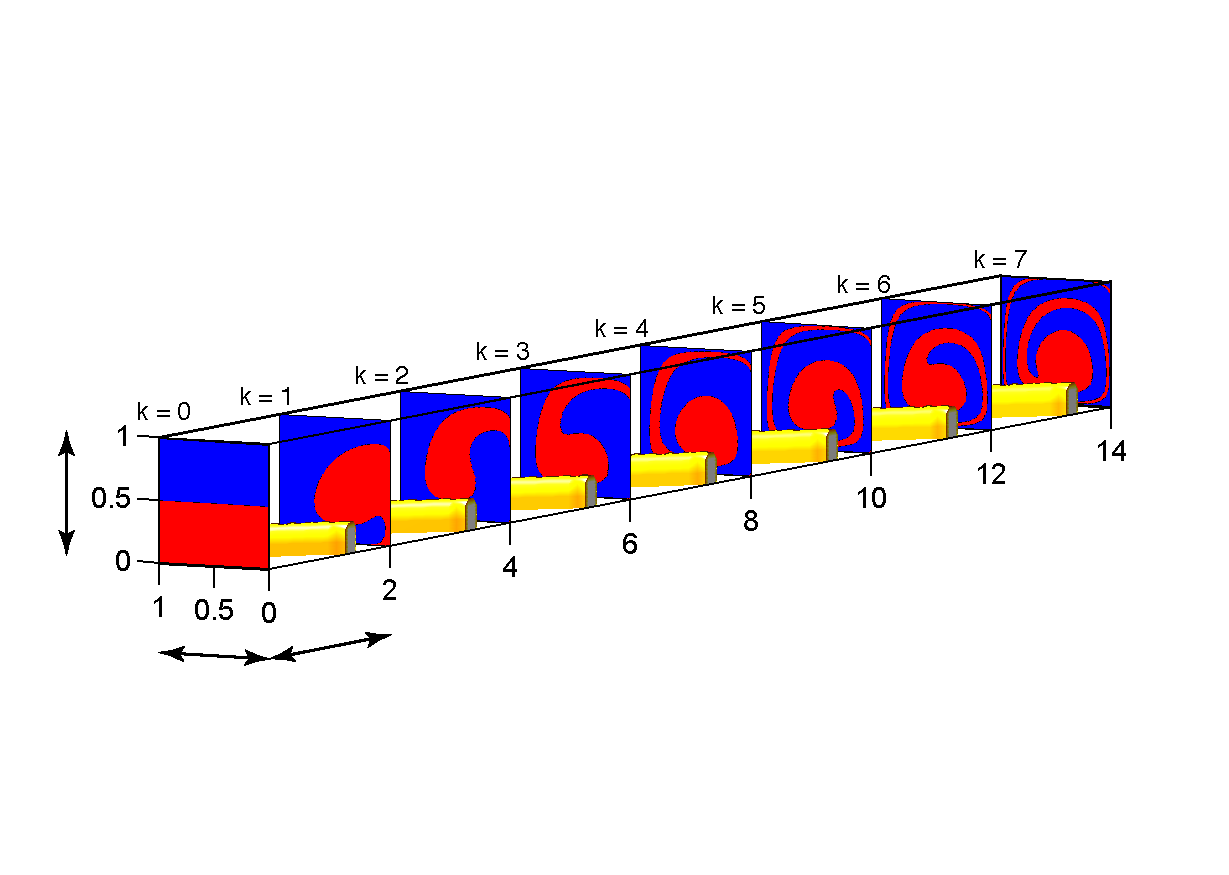
\includegraphics[width=0.8\textwidth,trim=0cm 3cm 0cm 2cm,clip]{mixingchannel}}
  \caption{\label{mixingchannel} The mixing channel. Liquids with two
    different colors are originally separated and injected from one
    side of the channel. Inside the channel there are periodic
    structures to stir the flow and produce transverse velocity
    components. The colored liquids then start to mix. In this figure,
    cross-sections of the color distribution are plotted every period
    of the structure.}
\end{figure}


As mentioned in the introduction, flow on the microfluidic
scale has $\text{Re}\sim 1$ and is thus highly laminar. A Stokes partial
differential equation is generally a reasonable model of the motion.
We simulate the flow by the generalized Stokes equation for
incompressible flow:
\begin{subequations}
  \label{stokes}
  \begin{align}
    \label{stokes1}
    ( -\nu\Delta + \alpha)u
    + \nabla p &= f, \\
    \label{stokes2}
    \mbox{div} u &= 0,
  \end{align}
\end{subequations}
where $u(\mathbf{x})$ and $p(\mathbf{x})$, which are both functions of
position $\mathbf{x}=(x,y,z)$, stand for the velocity and pressure
fields and $f$ is the body force that drives the flow. It has an
elliptic operator $-\nu\Delta + \alpha $ in which $\nu$ is the
kinematic viscosity and $\alpha(\mathbf{x})$ represents the inverse
permeability at $\mathbf{x}$. When $\alpha(\mathbf{x}) = 0 $ it is
just Stokes flow with viscosity $\nu$ and when $\nu=0$, one gets the
Darcy equation, which governs the flow in porous material with
permeability $\alpha^{-1}$. The liquids to be mixed are assumed to
have the same density and viscosity, which is true for
many applications when the liquids are solvents carrying different
reactants. This assumption is critical for our periodic setting 
to work, because now we can separate the color intensity field from 
the velocity field: the velocity field is stationary but the color 
intensity field has not. This allows us to use one period of velocity 
field repeatedly to carry the color intensity and observe the mixing process. 

 

\todo{MW: When I gave the talk on this last week there were a number
  of people confused because they thought that $\alpha$ was a scalar,
  rather than a scalar function of position. I think it might be worth
  making it clear that we have $u(x)$, $p(x)$ and $\alpha(x)$.}
\todo{TC: We use $x$ as one coordinate, so $u(x)$ is also confusing.
So I think $u(\mathbf{x})$ is better, and define $\mathbf{x}=(x,y,z)
$}

\todo{MW: Thinking about it further, the assumption that they liquids
  have the same density and viscosity is actually critical for our
  whole method, isn't it? If the flow field depended on the color then
  we couldn't do a period solve at all, as the equation would keep
  changing as we went further down the channel and the mixing state
  changed. So it's not just for simplicity that we assume that, but
  rather we really need to assume it. We should make this clear.}

\todo{TC:Agree. A sentence is added in above.}

We use a finite-difference method with staggered regular meshes to
solve the above equation. Assuming the finite-dimensional
approximation of the Laplace, gradient and divergence operators on the
given mesh are $L$, $G$, and $D$, the generalized Stokes equation can
be represented by
\begin{equation}
  \label{discretestokes}
  \left[\begin{matrix}
      -\nu L + \text{diag}(\bar{\alpha})H & G\\
             D                            &  0
    \end{matrix} \right]
  \left[\begin{matrix}
      \bar{u} \\ \bar{p}
    \end{matrix} \right]=
  \left[\begin{matrix}
      \bar{f} \\ \mathbf{0}
    \end{matrix} \right],
\end{equation}
where $\bar{u}$, $\bar{p}$, $\bar{\alpha}$, and $\bar{f}$ are vectors, representing
finite-dimensional approximations of $u$, $p$, $\alpha$ and $f$,
respectively. The linear operator $H$ maps the design parameters
$\bar{\alpha}$ to the directional $\bar{u}$ grids.



Let the number of grids in the $x$, $y$, and $z$ directions be $n_x$,
$n_y$, and $n_z$. We define $n_{\bar{u}} = 3n_x n_y n_z$, which is
roughly the size of $\bar{u}$, and $n_{\bar{\alpha}}=n_{\bar{p}} = n_x
n_y n_z$, which is roughly the size of $\bar{\alpha}$ and $\bar{p}$. A
typical case in our examples is $n_x = 144$, $n_y=24$, and $n_z=48$.



%%%%%%%%%%%%%%%%%%%%%%%%%%%%%%%%%%%%%%%%
\subsection{Topology optimization}
%%%%%%%%%%%%%%%%%%%%%%%%%%%%%%%%%%%%%%%%

We would like to optimize some objective function
$g(\bar{u},\bar{p},\bar{\alpha})$ over parameters $\bar{\alpha}$. The
direct approach would be to define an optimization problem
%\begin{align}
%\begin{split}
%  \text{minimize    } &
%  g(\bar{u},\bar{p},\bar{\alpha})\\
%  \text{subject to  } &\left[\begin{matrix} -\nu L + \text{diag} (\bar{\alpha}) H
%       & G \\ D & 0
%    \end{matrix} \right]
%    \left[\begin{matrix}
%      \bar{u} \\ \bar{p}
%    \end{matrix} \right]=
%    \left[\begin{matrix}
%     \bar{f} \\ \mathbf{0}
%    \end{matrix} \right], \\
%    &0 \le \bar{\alpha} \le \alpha_{\text{max}}
%    %& \mathbf{0}\le \bar{\alpha} \le \alpha_M\mathbf{1}
%\end{split}
%\end{align}
\begin{eqnarray}
\begin{array}{ll}
  \text{minimize}     & g(\bar{u},\bar{p},\bar{\alpha})\\
  \text{subject to  } &\left[\begin{matrix} -\nu L + \text{diag} (\bar{\alpha}) H
       & G \\ D & 0
    \end{matrix} \right]
    \left[\begin{matrix}
      \bar{u} \\ \bar{p}
    \end{matrix} \right]=
    \left[\begin{matrix}
     \bar{f} \\ \mathbf{0}
    \end{matrix} \right], \\
    &0 \le \bar{\alpha} \le \alpha_{\text{max}},
\end{array}
\end{eqnarray}
where $\alpha_{\text{max}}\in \mathbb{R}$ is a large number to approximate the minimum
permeability when $\alpha$ goes to infinity and the structure is
solid. The optimization problem has variables $\bar{u}$,
$\bar{p}$, and $\alpha_{\text{max}}$, and a large set of nonlinear equality
constraints that make the problem extremely hard to solve.

\todo{MW: I think that we can just say $0 \le \bar{\alpha} \le
  \alpha_{\text{max}}$ and say explicitly that $\alpha_{\text{max}}
  \in \mathbb{R}$. This notation is no more confusing that using $\le$
  on vectors in the first place, I think?}
\todo{TC: agree}

For a given $\bar{\alpha}$, we can solve \eqref{discretestokes} to
obtain $\bar{u}$ and $\bar{p}$ and there are no inequality constraints
on these two variables. We can thus rewrite the optimization and lump
the equality constraints into the objective function:
\begin{eqnarray}\label{topoptform}
  \begin{array}{ll}
    \text{minimize } & g(\bar{u}(\bar{\alpha}),
    \bar{p}(\bar{\alpha}), \bar{\alpha})
    \\ \text{subject to } & 0\le \bar{\alpha} \le \alpha_\text{max}.
  \end{array}
\end{eqnarray}
This formulation reduces the number of variables and eliminates the
nonlinear equalities, but it is now harder to evaluate the gradient of
the objective function, which we desire for efficiency in the
optimization algorithm. We will show later that an adjoint method can
be applied to efficiently compute the gradient.

%%%%%%%%%%%%%%%%%%%%%%%%%%%%%%%%%%%%%%%%%%%%%%%%%%%%%%%%
\subsection{Objective functions and a descent direction}
%%%%%%%%%%%%%%%%%%%%%%%%%%%%%%%%%%%%%%%%%%%%%%%%%%%%%%%%

%%%%%%%%%%%%%%%%%%%%%%%%%%%%%%%%%
\paragraph{Objective functions.}
%%%%%%%%%%%%%%%%%%%%%%%%%%%%%%%%%
Our goal is to optimize the shape of the structure inside the channel,
that is to find a vector $\bar{\alpha}$ such that the function
$g(\bar{u},\bar{p},\bar{\alpha})$ is locally minimized. The ideal
objective function is mixing length \cite{Stroock2002}: the channel
length required for the standard deviation of the color intensity on
the cross-section to drop by a given ratio. Unfortunately, this is a
very complicated function of the channel structure and there is no
clear way to find a descent direction to improve it. Hence, we use
several steps of heuristic designs to reduce the mixing length.

Two types of objective function will be considered in our
formulation. The first one is a function of the velocity field, which
is a very direct way to design the flow. In fact for most
applications, a linear function is good enough:
\begin{eqnarray}
  g_1(\bar{u},\bar{p},\bar{\alpha}) =
  \bar{c}^T\bar{u}.
\end{eqnarray}


\todo{MW: I don't like the notation below for $g_2$. Our $g$ objective
  functions should be functions of $u,p,\alpha$, not of
  $S_1,S_2$. Perhaps we can do something like define $S_u : [0,\ell_y]
  \times [0,\ell_z] \to [0,\ell_y] \times [0,\ell_z]$ to be the
  end-to-end particle map given by $u$, and then define
  $g_2(u,p,\alpha) = \|S^* - S_u\|$, or something like that?}

\todo{TC: fixed}

The second type of objective function
  measures the difference between two maps. Once the velocity is
  solved, the streamline can be calculated by numerical
  integration. Each of the streamlines connects a point on the $y$-$z$
  plane at $x=0$ to another point at $x=l_x$. The streamlines thus
  define an end-to-end flow map $S_u:[0,l_y]\times[0,l_z] \to
  [0,l_y]\times[0,l_z]$. Define $g_2(u,p,\alpha;S^*) = \|S^* - S_u\|$,
  where $S^*: [0,\ell_y] \times [0,\ell_z] \to [0,\ell_y] \times
  [0,\ell_z]$ is the desired end-to-end flow map and $\| \cdot \|$ is
  a distance measure of two maps $S_u$ and $S^*$. Suppose we know what
  the map we want is. The second type of objective function can then be
  applied to minimize the difference between the current map and the
  desired map. However, because each streamline needs to be calculated
  numerically, to define a map would be extremely hard. Therefore we
  simplify this objective function and let it measure the difference
  between a set of sample points on the $y$-$z$ plane. Let $(\bar{y}_0,\bar{z}_0)$
  be a set of sample points on the $y$-$z$ plane at $x=0$. We have
\begin{align*}
           (\bar{y}_e^*,\bar{z}_e^*)&= S^*(\bar{y}_0,\bar{z}_0), \\
           (\bar{y}_e,\bar{z}_e)    &= S_u(\bar{y}_0,\bar{z}_0). 
\end{align*}
We simply define $g_2$ as
\begin{eqnarray}
\label{g2}
           g_2(u,p,\alpha;S^*,\bar{y}_0,\bar{z}_0) = \|\bar{y}_e^*-\bar{y}_e\|^2 +  \|\bar{z}_e^*-\bar{z}_e\|^2,
\end{eqnarray}
where $\|\cdot\|$ is the $2$-norm of a vector. The above function is
a rough measure of how close the maps $S_u$ and $S^*$ are. In our
examples, $(\bar{y}_0,\bar{z}_0)$ is chosen as regular mesh grids on the $y$-$z$
plane.
%%%%%%%%%%%%%%%%%%%%%%%%%%%%%%%%%%%%%%%%%%%%%%%%%%%%%%%%%%%%%%%%%%%%
\paragraph{Adjoint method for $d g_1/d \mathbf{\bar{\alpha}} $.}
%%%%%%%%%%%%%%%%%%%%%%%%%%%%%%%%%%%%%%%%%%%%%%%%%%%%%%%%%%%%%%%%%%%%
To find a descent direction of $g_1$ with respect to $\bar{\alpha}$,
the adjoint method \cite{Jameson1999} is applied. Let $\bar{v} =
[\bar{u};\bar{p}]$. The variables $\bar{v}$ and $\bar{\alpha}$ satisfy
a set of constraints $R(\bar{v},\bar{\alpha})=0$, which is
stated in (\ref{discretestokes}). $d\bar{v}/d\bar{\alpha}$ has size
$(n_{\bar{u}}+n_{\bar{p}}) \times n_{\bar{\alpha}}$ (very large) and
is dense. We would like to calculate $d g_1/d\bar{\alpha}$ without
explicitly forming $d\bar{v}/d\bar{\alpha}$. The adjoint method is
designed for this situation. We begin with the total derivative of
$g_1$ and $R$ with respect to $\alpha$:
\begin{align*}
  \frac{dg_1}{d\bar{\alpha}} & =  \frac{\partial{g_1}}{\partial{\bar{\alpha}}}+
                                \frac{\partial{g_1}}{\partial{\bar{v}}} \frac{d\bar{v}}{d\bar{\alpha}},\\
  \frac{dR}{d\bar{\alpha}} & =  \frac{\partial{R}}{\partial{\bar{\alpha}}}+
                                 \frac{\partial{R}}{\partial{\bar{v}}} \frac{d\bar{v}}{d\bar{\alpha}}=0.
\end{align*}
From the second equation, we have
\begin{equation*}
  \frac{d\bar{v}}{d\bar{\alpha}}= -\left(\frac{\partial{R}}{\partial{\bar{v}}}\right)^{\dagger}\frac{\partial{R}}{\partial{\bar{\alpha}}}.
\end{equation*}
Substitute this into the first equation:
\begin{equation*}
   \frac{dg_1}{d\bar{\alpha}}  =  \frac{\partial{g_1}}{\partial{\bar{\alpha}}}-\frac{\partial{g_1}}{\partial{\bar{v}}} \left(\frac{\partial{R}}{\partial{\bar{v}}}\right)^{\dagger}\frac{\partial{R}}{\partial{\bar{\alpha}}}.
\end{equation*}
Let $\Phi = -\frac{\partial{g_1}}{\partial{\bar{v}}}
\left(\frac{\partial{R}}{\partial{\bar{v}}}\right)^{\dagger}$. Then
$\Phi$ satisfies
\begin{equation}
\label{adjointeq}
 \Phi \left(\frac{\partial{R}}{\partial{\bar{v}}}\right)^{T} = -\left({\frac{\partial{g_1}}{\partial{\bar{v}}}}\right)^T.
\end{equation}
The above equation is called the adjoint equation. More explicitly, the adjoint equation in our formulation is
\begin{equation}
\label{adjointeq2}
  \left[\begin{matrix}
     -\nu L + \text{diag}(\bar{\alpha})H   & G\\
     D               &  0
   \end{matrix} \right] \Phi^T =
  \left[\begin{matrix}
    -\frac{\partial{g_1}}{\partial{\bar{u}}}\\
    0
   \end{matrix} \right].
\end{equation}
After solving for $\Phi$, we can then evaluate $dg_1/d\bar{\alpha}$ by
\begin{equation}
\label{dg1dalpha}
  \frac{dg_1}{d\bar{\alpha}}  =  \frac{\partial{g_1}}{\partial{\bar{\alpha}}}+\Phi \frac{\partial{R}}{\partial{\bar{\alpha}}}.
\end{equation}
In our problem, $g_1$ does not depend on $\bar{\alpha}$ explicitly, so
the first term in the right-hand side of (\ref{dg1dalpha}) is zero. To
solve the adjoint equation (\ref{adjointeq2}), we need
$\partial{g_1}/\partial{\bar{u}}$, which is just $\bar{c}^T$ for
$g_1$.
%%%%%%%%%%%%%%%%%%%%%%%%%%%%%%%%%%%%%%%%%%%%%%%%%%%%%%%
\paragraph{Streamlines and $\partial g_2/\partial {\bar{u}}$.}
%%%%%%%%%%%%%%%%%%%%%%%%%%%%%%%%%%%%%%%%%%%%%%%%%%%%%%%
To find $d g_2/d \bar{\alpha}$, the above approach is still valid but
we need to form $\partial{g_2}/\partial{\bar{u}}$ first. Let the
solution of (\ref{discretestokes}) be the discrete velocity field
$\bar{u} = [\bar{u}_{x}; \bar{u}_{y}; \bar{u}_{z}]$. The velocity at
any point can be evaluated by linear interpolation. Given an initial
point $(0,y_{0},z_{0})$, a second-order Runge-Kutta method is applied to
find the streamline passing through it. Because both the interpolation
and Runge-Kutta method have linear weights on $\bar{u}$, we can write
down the following relations:
\begin{align*}
 x_e & =  k_{x}^T \bar{u}_{x}+0,\\
 y_e & =  k_{y}^T \bar{u}_{y}+y_{0},\\
 z_e & =  k_{z}^T \bar{u}_{z}+z_{0},
\end{align*}
where $k_{x},k_{y}$ and $k_{z}$ are the constant weighting vectors
generated by the numerical integration. $(x_e,y_e,z_e)$ is the point
where $(x_{0},y_{0},z_{0})$ maps to, assuming $x_e= \ell_x$.
$dy_e/d\bar{u}$ and $dz_e/d\bar{u}$ can be written as
\begin{align}
\begin{split}
 \frac{dy_e}{d\bar{u}} & =  \left[  \frac{\partial{y_e}}{\partial{x_e}} \frac{dx_e}{d\bar{u}_{x}},
                                        \frac{dy_e}{d\bar{u}_{y}},
                                        \mathbf{0}^T\right]
                                  =  \left[\frac{u_y(\mathbf{x}_e)}{(u_x(\mathbf{x}_e)}k_{x}^T,
                                        k_{y}^T ,\mathbf{0}^T    \right], \\
 \frac{dz_e}{d\bar{u}} & =  \left[  \frac{\partial{z_e}}{\partial{x_e}} \frac{dx_e}{d\bar{u}_{x}},
                                        \mathbf{0}^T,
                                        \frac{dz_{f}}{d\bar{u}_{z}}\right]
                                  = \left[\frac{u_z(\mathbf{x}_e)}{u_x(\mathbf{x}_e)_e}k_{x}^T,
                                        \mathbf{0}^T, k_{z}^T  \right],
\end{split}
\end{align}
where $\mathbf{x}_e= (x_e,y_e,z_e)$ and $u_x(\mathbf{x}_e),u_y(\mathbf{x}_e)$ and $u_z(\mathbf{x}_e)$ can also be evaluated by interpolation. Hence
$dg_2/d\bar{u}$, where $g_2$ has the form of equation (\ref{g2}), can
be written as
\begin{eqnarray}
   \frac{\partial g_2}{\partial \bar{u}} = \sum_{y_e} \frac{\partial{g_2}}{\partial{y_e}} \frac{dy_e}{d\bar{u}}+
                                    \sum_{z_e} \frac{\partial{g_2}}{\partial{z_e}}\frac{dz_e}{d\bar{u}}.
\end{eqnarray}
%%%%%%%%%%%%%%%%%%%%%%%%%%%%%%%%%%%%%%%%%%%%%%%%%%%%%%%%
\subsection{The gradient-based method}
%%%%%%%%%%%%%%%%%%%%%%%%%%%%%%%%%%%%%%%%%%%%%%%%%%%%%%%%
We use a gradient-based method to solve (\ref{topoptform}):

\begin{tabular}{ll}
\textbf{Algorithm} &\\
\hline
\textbf{given}  &    a starting vector $\bar{\alpha}^0$, $k=0$, $\star=1$ or $2$. \\
\textbf{repeat} &    1. solve (\ref{discretestokes}) for the velocity field.   \\
                &    2. solve the adjoint equation (\ref{adjointeq2}) and find $\frac{dg_\star}{d\bar{\alpha}}$. \\
                &    3. $\bar{\alpha}^{k+1} = 
                        \bar{\alpha}^{k}-\frac{dg_\star}{d\bar{\alpha}} \times \text{stepsize}$.   \\
                &    4. project the components of $\bar{\alpha}^{k+1}$ outside $[0,\alpha_\text{max}]$ to $0$ and $\alpha_\text{max}$. \\
                &    5. $k = k+1$.\\
\textbf{until}  &     stop criterion is satified. \\%$\max(\alpha) >\alpha_\text{max}$\\
\hline
\end{tabular}

\vspace{0.5cm}
 Here are some points we need to make:
\begin{itemize}
\item  For all of our examples, we use $\bar{\alpha}^0 = \mathbf{0}$ as the initial material distribution, and there is no total material constraint.
\item  In step $4$, the projection to zero is necessary because material with negative inverse permeability does not make physical sense.
\item  In our formulation, to evaluate the objective function is very expensive, so there is no line search in this algorithm. A fixed step size is used, and the step size is tuned by trial.  
\item  The stop criterion we use is
       \begin{eqnarray}
         \left\|\frac{\bar{\alpha}^k}{\|\bar{\alpha}^k\|_2}-\frac{\bar{\alpha}^{k+1}}{\|\bar{\alpha}^{k+1}\|_2}\right\|_2 < \epsilon.
       \end{eqnarray}
       For all of our examples, we observe that when the structure is formed,
the projection of the negative gradient direction gradually aligns
with the current $\bar{\alpha}^k$ direction. So the structure shape does not
change but the permeability keeps decreasing. Hence this stop criterion is handy in finding the structure shape.
\end{itemize}
%%%%%%%%%%%%%%%%%%%%%%%%%%%%%%%%%%%%%%%%%%%%%%%%%%%%%%%%%%%%%%%%%%%%%%
%%%%%%%%%%%%%%%%%%%%%%%%%%%%%%%%%%%%%%%%%%%%%%%%%%%%%%%%%%%%%%%%%%%%%%
\section{Simulation: a probabilistic model of the structured channel}
\label{sec:simu}
%%%%%%%%%%%%%%%%%%%%%%%%%%%%%%%%%%%%%%%%%%%%%%%%%%%%%%%%%%%%%%%%%%%%%%
%%%%%%%%%%%%%%%%%%%%%%%%%%%%%%%%%%%%%%%%%%%%%%%%%%%%%%%%%%%%%%%%%%%%%%
In this section we talk about given the periodic velocity field, how to build a Markov Chain model to simulate the mixing process. We first need to introduce two operators and their physical meaning in this application, and then the diffusion issue is considered. 
%%%%%%%%%%%%%%%%%%%%%%%%%%%%%%%%%%%%%%%%%%%%%
\subsection{The operator to evolve the color}
%%%%%%%%%%%%%%%%%%%%%%%%%%%%%%%%%%%%%%%%%%%%%
\todo{TC: We have defined $\mathbf{x}=(x,y,z)$. Now we use
$\mathbf{y}=(y,z)$. }

For a measure space $(Y,\mathcal{A},\mu)$, let $\mu$ be the
Lebesgue measure.  
\begin{definition} {\bfseries (Perron-Frobenius operator)}
Let $\omega \in L^1(Y)$, and suppose that for every $A \in \mathcal{A}$ the operator
$P_S:L^1(Y) \to L^1(Y)$ satisfies
  \begin{eqnarray}
    \int_A (P_S \omega)(\mathbf{y})\mu(d\mathbf{y}) = \int_{S^{-1}(A)} \omega(\mathbf{y})\mu(d\mathbf{y}).
  \end{eqnarray}
$P_S$ is the Perron-Frobenius operator associated with $S$.
\end{definition}
The Perron-Frobenius operator evolves a probability distribution.
\begin{definition} {\bfseries (Koopman operator)}
Let $f \in L(Y)^\infty$. The operator $U_S:L^{\infty}(Y) \to
L^{\infty}(Y) $ defined by
 \begin{eqnarray}
 U_Sf(\mathbf{y}) = f(S(\mathbf{y}))
 \end{eqnarray}
is called the Koopman operator associated with $S$.
\end{definition}
The Koopman operator is the adjoint of the Perron-Frobenius operator, and they are both linear operators. Because they are a pair of adjoint operators, suppose
$U_{S^{-1}}$ has the matrix representation $A$, $P_{S^{-1}}$ is thus $A^T$. Hence, once we find
either of the operators, the other is easily obtained.

Now we would like to model one period of the mixing channel and repeatedly use this model to evolve the color intensity on the cross-sections of the channel. Letting $Y = [0,\ell_y]\times[0,\ell_z]$, one can define an invertible map $S:Y\to Y$ by integrating
the streamlines from $x=0$ to $x=\ell_x$. We represent the color intensity as a function $f^k : Y \to [0,1] $ on cross-section $k$, and want to find the operator to map the color function from cross-section $k$ to $k+1$ with fixed distance $\ell_x$ (remember the velocity field is periodic). A direct choice would be to interpret the color function as a probability density and evolve it by $P_S$. However, this is physically incorrect because ${\int\int}_Y f^k \,dy\,dz$ does not stay constant for different $k$ because of the non-constant flow velocity over $Y$. Let the stationary $x$-directional flow velocity on the cross-sections $x=0, l_x, 2l_x, \ldots$ be $v_x: Y \to \mathbb{R}$. One has the following conservation:
\begin{equation}
\label{fvc}
  {\int\int}_Y f^k v_x \,dy\,dz = {\int\int}_Y f^{k+1} v_x \,dy\,dz \text{  , for }k=0,1,2,\ldots,
\end{equation}
which says the total ``color'' flowing in and out of one period of the channel has to be constant. Thus the correct choice to evolve the color intensity would be $U_{S^{-1}}$. One can check that using $U_{S^{-1}}$ to evolve $f^k$ satisfies the above equality because $v_x$ is an invariant measure under map $S$. 


%Let $Y = [0,\ell_y]\times[0,\ell_z]$ and define $\mathbf{y}=(y,z)$, one can
%define an invertible map $S:Y\rightarrow Y$ by integrating the
%streamlines from $x=0$ to $x=\ell_x$. Let the color intensity on $Y$ when
%$x = 0$ and $x = \ell_x$ be scalar functions $f_0,f_{x_l}: Y \rightarrow
%[0,1]$, and ${u_x|_{Y_0}}:Y \rightarrow \mathbb{R}$ the $x$ direction
%velocity on $Y$ when $x=0$ or $\ell_x$(periodic boundary condition). One
%can think ${u_x|_{Y_0}}(y,z)$ as how many flow particles flow through
%the point $(0,y,z)$ or $(\ell_x,y,z)$ per unit time. Each flow particle
%is colored and the color can be represented by a number between $0$
%and $1$. Thus $f_0(y,z)$ is the color we see on $(0,y,z)$ and is
%interpreted as the average color of the particles that flow through
%$(0,y,z)$. Note this quantity has nothing to do with
%${u_x}|_{Y_0}(y,z)$ (flowing faster does not make the color deeper!),
%but the total ``color'' that flows in and out the channel has to be
%conserved, i.e., we have

% \begin{equation}
% \label{fvc}
%          \int_Y f_0 {u_x}|_{Y_0} d\mathbf{x}  =  \int_Y f_{\ell_x} {u_x}|_{Y_0} d\mathbf{x} = C
% \end{equation}
%where $C$ is a constant. This says that it is not appropriate to
%interpret the color intensity as a probability distribution. Instead,
%if we think the velocity of the flow particles on $Y$ has distribution
%$\bar{\omega} = \frac{{u_x}|_{Y_0}}{\int_{Y}{u_x}|_{Y_0}d\mathbf{y}}$
%and is invariant, the natural choice of the operator to satisfy
%(\ref{fvc}) and evolves the color intensity forward in time is
%$U_{S^{-1}}$: the Koopman operator of the map $S^{-1}$.



%%%%%%%%%%%%%%%%%%%%%%%%%%%%%%%%%%%%%%%%%%%%%
\subsection{Diffusion issue}
%%%%%%%%%%%%%%%%%%%%%%%%%%%%%%%%%%%%%%%%%%%%%

Suppose inside the mixing channel, the color is diffusive with
diffusivity $D$, and we are interested in the color intensity on the
cross-sections of the channel at each end of the period ($f^k$). This
corresponds to solving the steady state Advection-Diffusion equation
 \begin{eqnarray}
 \label{ade}
        u \cdot \nabla \phi = D \Delta \phi
 \end{eqnarray}
with suitable boundary conditions, where 
$\phi(\mathbf{x})$ is the color intensity and $u(\mathbf{x})$ is the $3$-D
periodic velocity field. One should have $f^k = \phi(k\ell_x,y,z)$ for 
all $k$. Solving (\ref{ade}) is not any harder than
solving the velocity field, but $\phi$ is certainly not periodic even if
$u$ is, so it is a much larger problem than (\ref{stokes}). We
would like to use $U_{S^{-1}}$ to approximate the solution of
(\ref{ade}) on $x = k\times \ell_x$ for $k=0,1,2,\ldots$. However, the map
$S$ contains no molecular diffusion information, so its $U_{S^{-1}}$
does not really mix colors. Thus we cannot just use $U_{S^{-1}}$ or
its matrix form $A$ to simulate the mixing process of the mixing
channel. To make the process diffusive, the diffusion needs to be put
manually into the operator. In fact, in practice it is impossible to
find the infinite-dimensional $A$. One can only approximate $A$ by a
finite-dimensional Markov operator $A_n\in \mathbb{R}^{n\times n}$
such that $\lim_{n \rightarrow \infty}A_n =A$, and it is always
irreducible and hence diffusive. The way we find the approximate $A$
is through optimal model reduction \cite{Beck2007, Froyland2001,
Froyland1999}. We discretize the domain $X$ into regular $m_y \times
m_z$ square mesh grids with size $h$ to form a reduced space
$\mathbb{R}^{m_y m_z}$. Let $n=m_y m_z$ and each of the grid be named
$a_i$, for $i=1,2,\ldots,n$. Each $a_i$ represents a new state in the
reduced space. To find $A_n$ in the reduced space, we need a map (an
observer) $g_n: f(\mathbf{y}) \mapsto f_n $ such that
\begin{eqnarray}
  (f_n)_i = (g_n(f(\mathbf{y})))_i = \int_{a_i} f(\mathbf{y}) \mu(d\mathbf{y})  \mbox{, for }i = 1 \mbox{ to } n.
\end{eqnarray}
For any $f$ and $f_n = g_n(f)$, the optimal reduced model of $A$ is
$A_n$ such that
\begin{eqnarray}
\label{objfunction}
  A_n f_n = \operatorname*{argmin}_{{f'_n}} \| {f'_n} -g_n(Af) \|_{\text{diag}(\sqrt{\bar{\omega}_n})},
\end{eqnarray}
where  $\bar{\omega}_n =g_n(\bar{\omega})= g_n(v_x/|v_x|)$ is the invariant
distribution of the Markov transition matrix $A_n$. In this case, the
optimal $A_n\in \mathbb{R}^{n \times n}$ satisfying
(\ref{objfunction}) can be calculated explicitly as
  \begin{eqnarray}
    \label{Anij}
    (A_n)_{ij} =  \frac{\bar{\omega}(S(a_j)\cap a_i)}{\bar{\omega}(a_j)}.
   \end{eqnarray}
The color intensity is thus evolved by
\begin{eqnarray}
     f_n^{k+1} = A_n f^k_n,
\end{eqnarray}
and clearly, we have a discrete version of (\ref{fvc}).
\begin{eqnarray}
     (f_n^{k+1})^T \bar{\omega}_n=  (f^k_n)^T \bar{\omega}_n.
\end{eqnarray}




To evaluate ($\ref{Anij}$) requires the calculation of $S^{-1}(a_j)$,
finding the area intersection, and integration over a non-uniform
measure $\bar{\omega}$ (the velocity profile $v_x$ on the cross-section). For most of the maps, these steps can only be done numerically. This $A_n$ is an approximation of the infinite-dimensional operator $A$, and has numerical diffusion $D_0 \sim h^2$
per iteration. By choosing a different grid size we can adjust the
numerical diffusion of the operator $A_n$. When the grid size is small
($n>100^2$) it is very hard to evaluate (\ref{Anij}); hence a numerical
approximation of the area is used.


Figure \ref{mixingcrosssection} is a demonstration of the $A_n$
operator. We use $n= 100^2, 200^2$, and $400^2$ to approximate $A$,
and simulate the mixing channel shown in Figure \ref{mixingchannel}.
The channel has dimension $(\ell_x,\ell_y,\ell_z) =
(0.02,0.01,0.01)\,\text{cm}$ for one period. Liquids with color black
(intensity $1$) and white (intensity $0$) are injected from one side
of the channel where the upper half of the liquid is white and the
lower half is black. For comparison we also use streamlines to evolve
the black/white boundary to simulate the situation without diffusion.
The results show that the model does capture how the boundary evolves
accurately even for very coarse grids. The only difference between
coarse and fine grids is in the diffusion part.

In our later numerical examples, to obtain accurate diffusion of the
operator, we use a very fine grid size to make the numerical diffusion
much smaller than the actual diffusion we want. A 2-D FFT/IFFT
scheme is then applied to add more diffusion in the frequency domain after
each iteration. One should note that the $f^k$ given by this
probabilistic model is by no means an accurate solution of
(\ref{ade}). However, it does capture the most important factors in
chaotic mixing: stretching, folding, and the molecular diffusion. We
demonstrate later by examples that this approximation agrees
well with experimental results.


  \begin{figure}
    \centerline{
    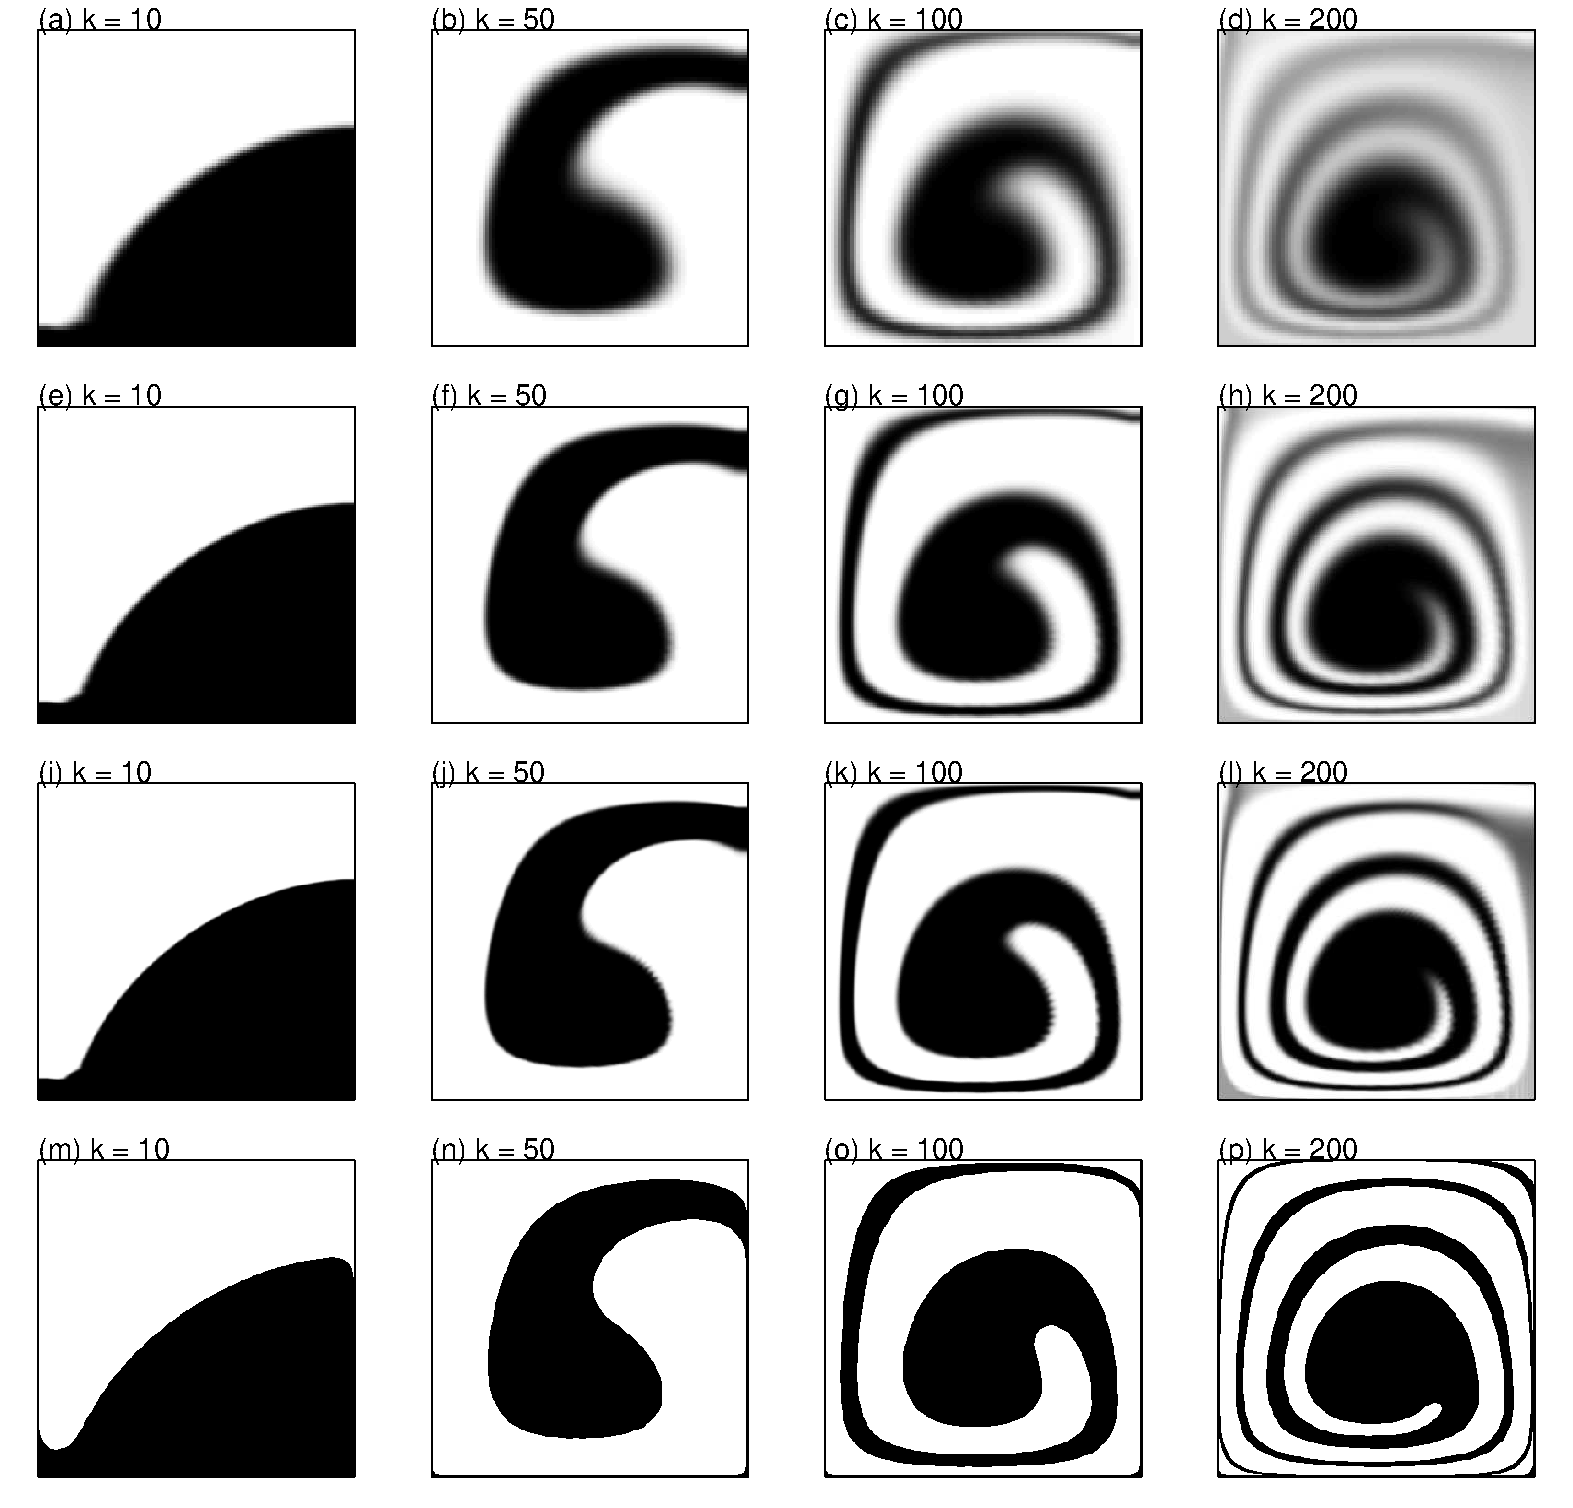
\includegraphics[width=1\textwidth]{mixingchannelcrossdiffusion}}
    \caption{The cross-sections of the mixing channel at iterations $k=10, 50, 100$, and $200$. Figures (a)--(d) have resolution $100 \times 100$ ($A_{100^2}$), (e)--(h) have resolution $200 \times 200$ ($A_{200^2}$), and (i)--(l) have resolution $400 \times 400$ ($A_{400^2}$). Figures (m)--(p) we use streamlines to evolve the black/white boundary to simulate the mixing channel without any diffusion.}
  \label{mixingcrosssection}
  \end{figure}



%%%%%%%%%%%%%%%%%%%%%%%%%%%%%%%%%%%%%%%%%%%%%%%%%%%%%%%%%%
%%%%%%%%%%%%%%%%%%%%%%%%%%%%%%%%%%%%%%%%%%%%%%%%%%%%%%%%%%
\section{Results}
\label{sec:topoptresults}
%%%%%%%%%%%%%%%%%%%%%%%%%%%%%%%%%%%%%%%%%%%%%%%%%%%%%%%%%%
%%%%%%%%%%%%%%%%%%%%%%%%%%%%%%%%%%%%%%%%%%%%%%%%%%%%%%%%%%

In all of our simulations, we use $\nu = 0.01 \, \text{g}
\,\text{cm}^{-1}\, \text{s}^{-1}$, $\ell_y,\ell_z \sim 0.01\,\text{cm}$ and
adjust the body force to make the average $x$ velocity around
$1\,\text{cm}\, \text{s}^{-1}$ so that $\text{Re} =U\ell/\nu\approx 1$.
The grid size we use to discretize the channel cross-section is
$h=1.25\times 10^{-5}\text{cm}$, which corresponds to $8 \times 10^4$ grids per
centimeter. The numerical diffusion caused by this discretization is
$D_0 \sim h^2 =1.5\times 10^{-10}\,\text{cm}^2$ per period of the
channel. A $2$-D FFT/IFFT scheme is applied to control the
diffusion further. The diffusion added by the FFT/IFFT scheme is at least
$10^{-9}\,\text{cm}^2$ per period, and hence $D_0$ is negligible.

To decide $\text{Pe}$, for example, when $\ell=\ell_y=\ell_z=0.01\,\text{cm}$,
let $\ell_x =0.02 \,\text{cm}$ $U=1 \, \text{cm} \, \text{s}^{-1}$, and
diffusivity be $10^{-9}\,\text{cm}^2$ per period of the channel. Then
$D = 10^{-9}\times U/\ell_x =
5\times10^{-8}\,\text{cm}^2\,\text{s}^{-1}$, and $\text{Pe} = U\ell/D =
2\times10^5$. Note that the mesh we use to solve the velocity fields
($n_x,n_y,n_z$) is different from the mesh to generate $A_n$ ($n_A$).


%%%%%%%%%%%%%%%%%%%%%%%%%%%%%%%%%%%%%%%%%%%%%%%%%%%%%%%%%%%%%%%%%%%%%%%%%%
\subsection{Maximizing the downward velocity at the center of the channel}
%%%%%%%%%%%%%%%%%%%%%%%%%%%%%%%%%%%%%%%%%%%%%%%%%%%%%%%%%%%%%%%%%%%%%%%%%%
This example is to demonstrate the use of the objective function $g_1$
and address the porous material issue. The mixing channel has
dimension $(\ell_x,\ell_y,\ell_z) = (0.02,0.01,0.01)\,$cm per period, and is
discretized into $(n_x,n_y,n_z)=(64,32,32)$ grids. We set $c$ to
maximize the downward (negative $y$ direction) velocity inside the
block $[0,\ell_x]\times[0.3\ell_y,0.7\ell_y]\times[0.3\ell_z,0.7\ell_z ]$. The
optimization runs for $46$ iterations and the structure shape is
formed as shown in the right of Figure \ref{example1structure}. Seven
of the streamlines are plotted as well. From the streamline, it is
easy to see that our objective is achieved. In the left of Figure
\ref{example1structure} we plot how $\bar{\alpha}$ grows versus iterations on
a line. This plot says that the material can be added in or taken out
by the algorithm, so the gradient direction does change, and we are
not solving a trivial problem. Moreover, one can clearly observe that
the material gradually forms a black/white solution such that
eventually $\bar{\alpha}$ only takes the value $0$ or $\alpha_\text{max}$.


  \begin{figure}
    \centerline{
     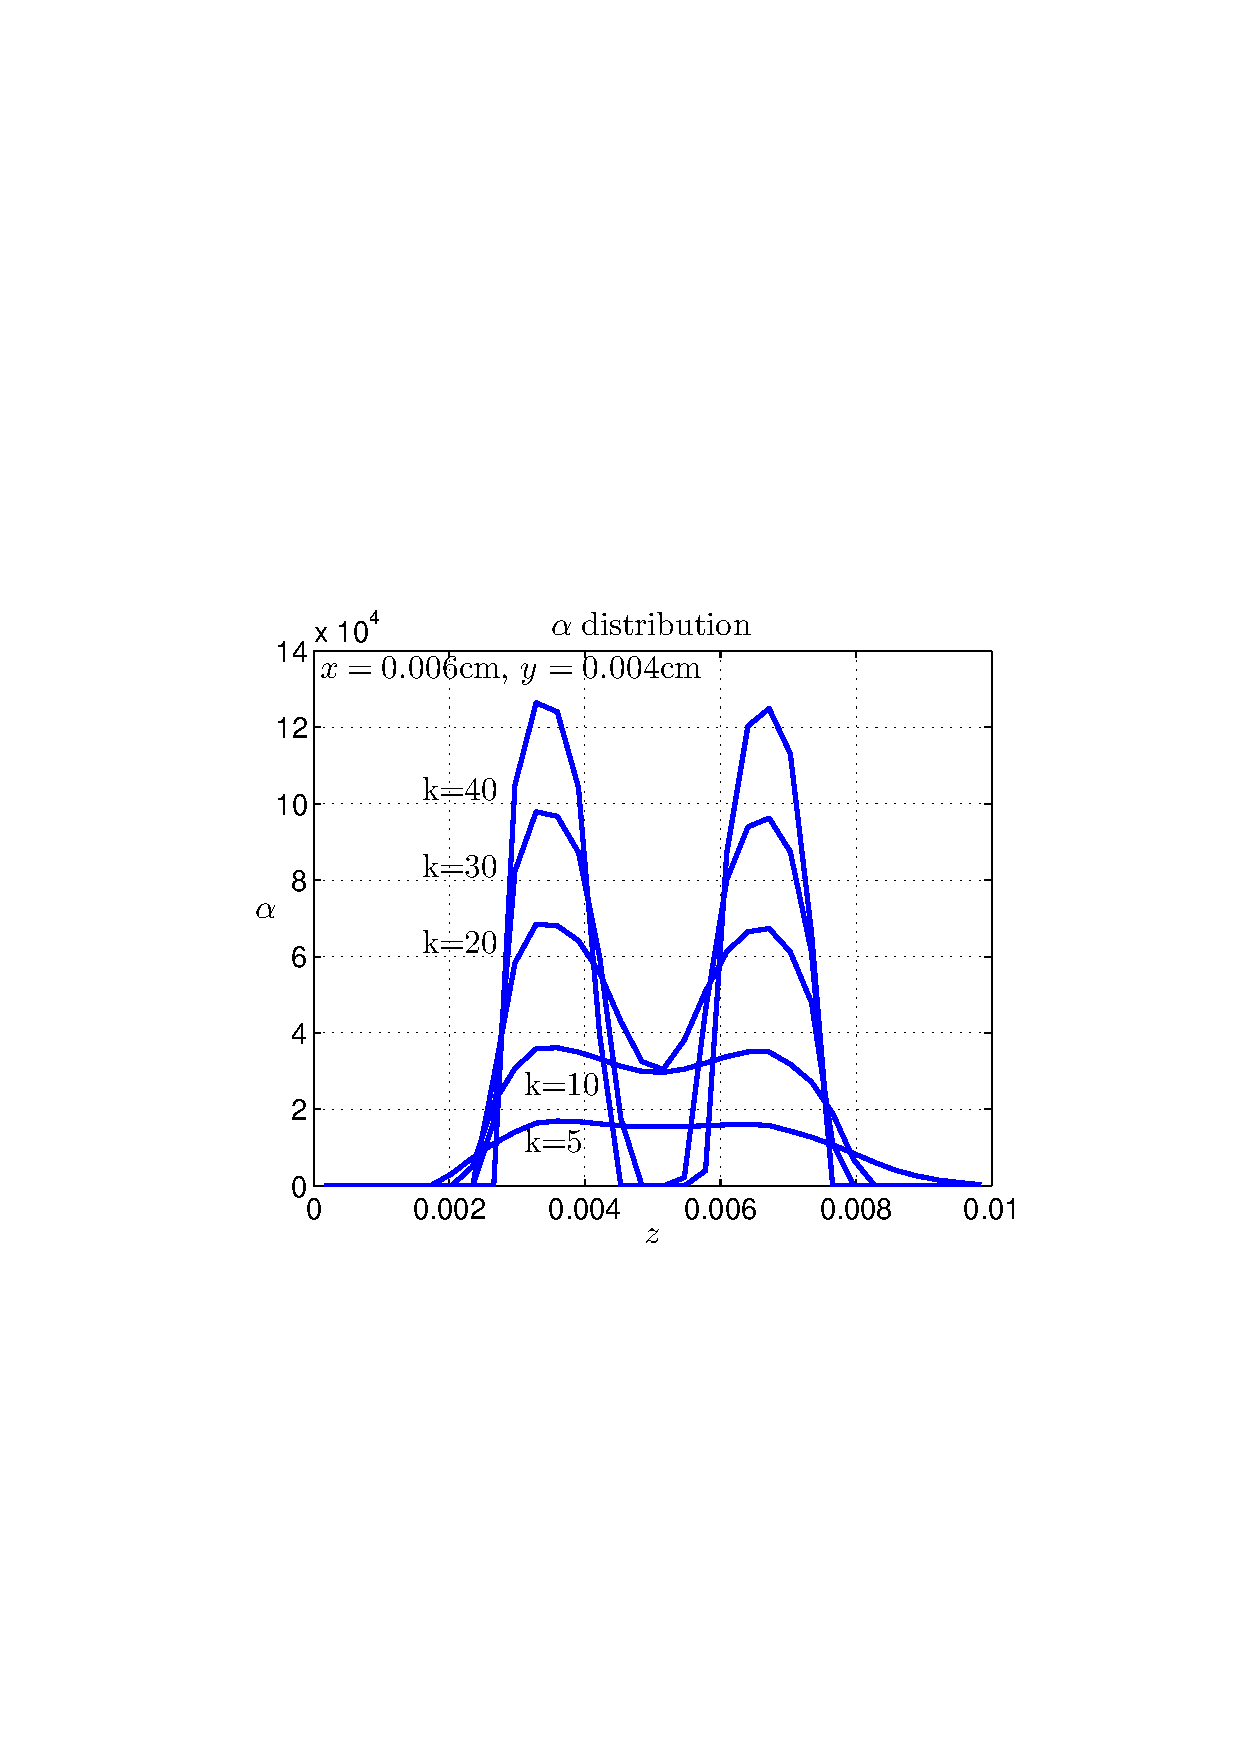
\includegraphics[width=0.5\textwidth]{example1alphaevolve}
     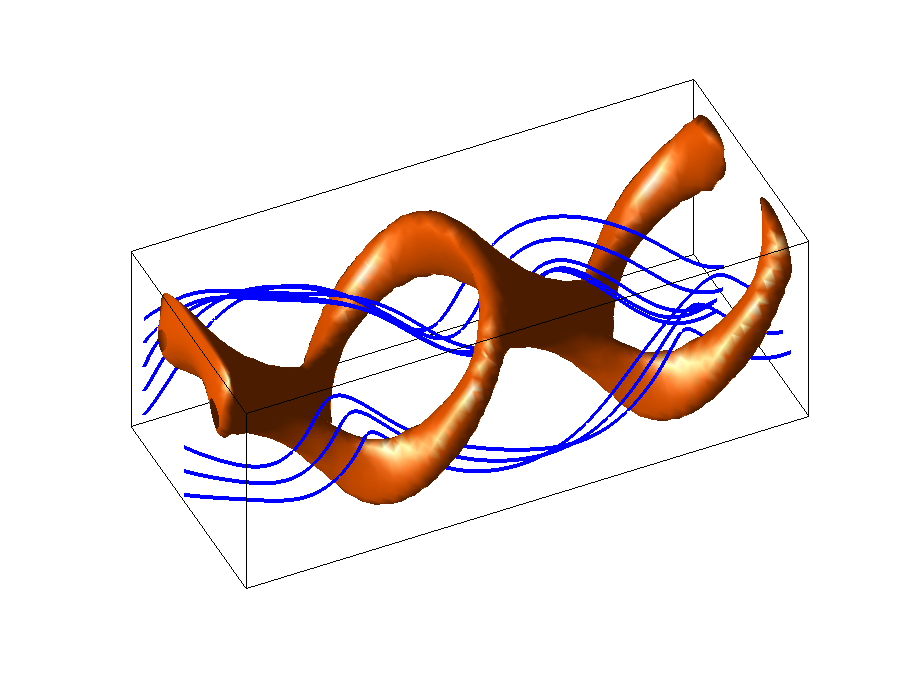
\includegraphics[width=0.5\textwidth]{example1structure2}}
    \caption{\label{example1structure} The left figure shows how $\alpha$ grows versus iteration on a line. It demonstrates that the material can be added in or taken out. The structure to maximize the downward velocity at the center of the channel after $46$ iterations is shown in the right figure. }
  \end{figure}

We use the simulation method we proposed to simulate this
system. The result is shown in Figure \ref{example1simulation}. The
system is clearly doing the right thing (maximizing the downward
velocity at the center of the channel).

  \begin{figure}
    \centerline{
     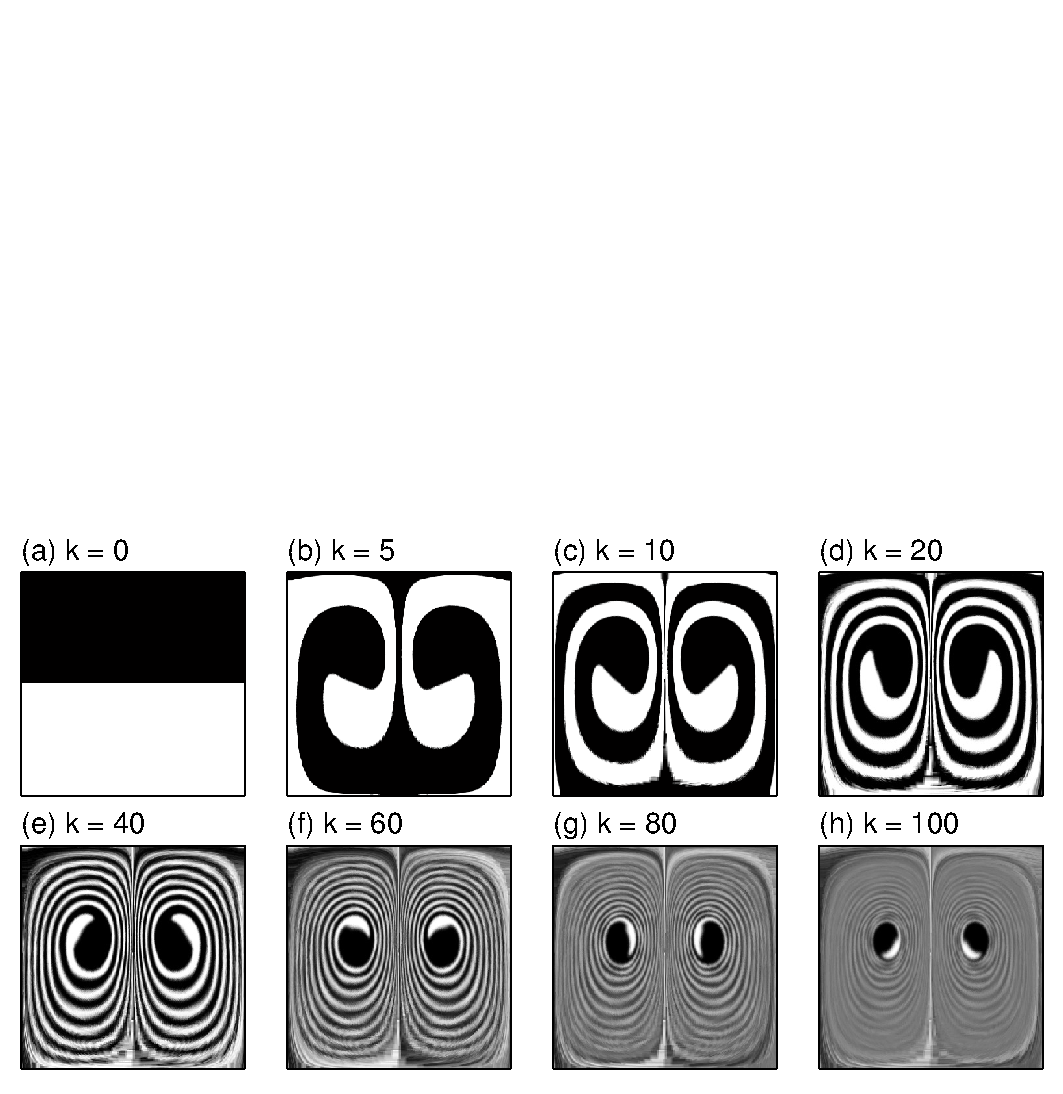
\includegraphics[width=1\textwidth,trim=0cm 0cm 0cm 7cm,clip]{example1simu}
     }
    \caption{\label{example1simulation} The cross-section simulation of the structured channel shown in Figure \ref{example1structure}.}
  \end{figure}

%%%%%%%%%%%%%%%%%%%%%%%%%%%%%%%
\subsection{A mixing channel }
%%%%%%%%%%%%%%%%%%%%%%%%%%%%%%%
In this example, we want to show how the use of a $g_1$ kind of
objective function can help us to design a mixing channel to realize
chaotic mixing. Stroock, et al.\ \cite{Stroock2002} proposed a
staggered herringbone mixer composed of two sequential
regions of ridges; the direction of asymmetry of the herringbones
switches with respect to the center-line of the channel from one region
to the next. The herringbone structure is fabricated with two steps of
photolithography and is located on the floor of the poly channel.
Experiments show that the length of the channel required for mixing
grows only logarithmically with $\text{Pe}$, instead of linearly as
in a smooth channel. The goal of the herringbone structure is to
produce transverse flows for which we can further optimize by the
$g_1$ objective function.

The mixing channel has dimension $(\ell_x,\ell_y,\ell_z) =
(0.06,0.01,0.02)\,$cm per period and is discretized into
$(n_x,n_y,n_z)=(144,24,48)$ grids. We set $c$ to maximize the downward
(negative $y$ direction) velocity inside the block
$[0,\ell_x]\times[0,\ell_y]\times[\frac{2}{6}\ell_z,\frac{5}{6}\ell_z ]$, which
can produce larger and smaller vortices. We consider two
scenarios: the material is restricted to be on the bottom of the
channel (the block $[0,\ell_x]\times[0,0.2\ell_y]\times[0,\ell_z]$), and the
material can be put anywhere inside the channel. The optimal
structures of both scenarios, as shown in Figure
\ref{example2structureNew}, contain several periods of (almost) the
same structure. The same pattern repeats four times in the first case
and three times in the second case. One can see that for the first
scenario, the optimal structure is also a herringbone type, but has a
higher frequency for the smaller vortex. For the second scenario, the
structure is formed by much more material and also tends to have a
higher frequency for the smaller vortex.


Just like in the previous example, one can simulate how the channel
mixes the colors by the Markov Chain model. However, in order to
produce chaotic mixing, the mixer has to be composed of two sequential
regions that are symmetric with respect to the plane
$z=\frac{1}{2}\ell_z$, and this breaks the periodic boundary condition
assumed in obtaining the Markov Chain. In order to perform a correct
simulation, one needs to solve the flow field for a full cycle of
channel.

Let us focus on the first scenario. Since the same structure repeats
four times in the solution, we take one of them and call it ``L''
(with dimension $(\ell_x,\ell_y,\ell_z)=(0.015,0.01,0.02)\,)$cm. The symmetric
structure of ``L'' is thus called ``R''. One can build an $n$-cycle
channel by connecting $n/2$ L structures and $n/2$ R structures
together. It thus has the period $0.015n\,\text{cm}$. For fixed
$\text{Pe}=1.2 \times 10^4$, we solve the flow field for different
$n$-cycles with $n=6$, $8$, $10$ and $12$, and find that when $n=8$,
the channel has the best mixing. Hence in Figure
\ref{example2trajectory}, the 8-cycle mixing channel is used to
perform the simulation with different $\text{Pe}$. We adjust
$\text{Pe}$ by changing the FFT/IFFT diffusivity between each
$8$-cycle ($0.12\,\text{cm}$). The trajectories have the same tendency
as the experiment results in the Figure 3(D) in \cite{Stroock2002}.
Define mixing length ($x_{90}$) as the channel length required for the
standard deviation to drop to $0.05$ (shown by a dashed line in Figure
\ref{example2trajectory}). The mixing length grows linearly with
$\log(\text{Pe})$, which also matches the experiments done in
\cite{Stroock2002}.


In Figure \ref{example2simu} we show some cross-sectional plots of two of
the simulations in Figure \ref{example2trajectory}, where the channel
is 8-cycle and $\text{Pe}$ are $1.2\times10^6$ and $1.2\times10^9$,
respectively. The first four plots of each case show the cross-section
at the end of the 1st to the 4th cycle, and the last plot for each
case shows the cross-section at the end of the 9th cycle. From this
comparison one can clearly see how the chaotic mixing protocol helps
color mixing even when diffusion is very small.


As for the 3-D structure, the best $n$-cycle we find is $n=2$
($\ell_x=0.04\, \text{cm}$) because this structure stirs the flow a lot.
To further compare our optimized structures and the design in
\cite{Stroock2002}, we also perform a simulation of Stroock's
staggered herringbone mixer. The mixing length versus
$\log({\text{Pe}})$ for the three simulations and the experiment data
given in \cite{Stroock2002} are plotted in Figure
\ref{example2mixinglength}. One can see that our simulation ($\times$)
has a longer mixing length comparing with the experiment
data ($\lozenge$) when $\text{Pe}$ is small, and they agree well when
$\text{Pe}\approx 10^6$ ($\log(\text{Pe})=14$). For even larger
$\text{Pe}$, the simulation is a reasonable linear extension of the
experiment data. As for the optimal mixing channel we suggest
($\square$ for the herringbone, and $\bigcirc$ for the 3-D structures), they
both significantly outperform Stroock's design.

In Figure \ref{example2crosscompare} (a) and (b), for
$\log(\text{Pe})=14$, the cross-section at the end of the $5$-th cycle
of our optimal herringbone solution and Stroock's design are plotted.
One can compare the simulation in Figure \ref{example2crosscompare}(b)
with Figure 3(C) in \cite{Stroock2002} to see how similar they are.
This justifies our Markov Chain model is valid when the diffusion is
small.


For the above two cases, the average flow velocity in the $x$
direction are both around $1.2\, \text{cm} \,\text{s}^{-1}$. We use
the same body force for the simulation of the optimal $3$-D structure,
and adjust the diffusivity to make $\log(\text{Pe})=14$. The optimal
$3$-D structure has a much shorter cycle length
($\ell_x=0.04\,\text{cm}$). Hence we plot the cross-section of it at the
end of $15$-th cycle in Figure \ref{example2crosscompare}(c). It shows
that when $x=0.6\, \text{cm}$, the colors have a much better mixing
than both herringbone type channels. However, since there is more
material stuffed inside the channel, for the same body force, the
average flow velocity in the 3-D structure channel is only $0.2\,
\text{cm} \,\text{s}^{-1}$--six times slower than the herringbone type
channels. Hence when we plot the cross-section of this mixing channel
at time $t=0.7s$ in Figure \ref{example2crosscompare}(d), it is not
significantly better than the other two channels at $t=0.5\,s$ and
$t=0.6\,s$. This says if one cares more about mixing time rather than mixing length, 
the $3$-D structure may not be the preferable choice. 

\todo{TC: Figure \ref{example2structureNew} needs to correct the unit.}

%%%%%%%%%%%%%%%%%%%%%%%%%%%%%%%%%%%%%%%%%%%%%%
% structure plot
  \begin{figure}
    \centerline{
     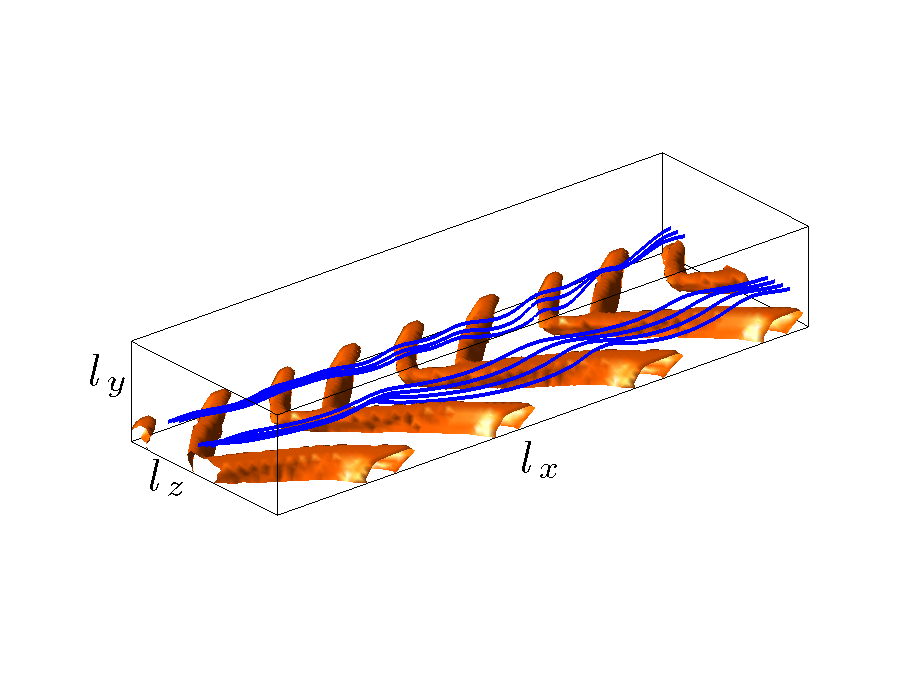
\includegraphics[width=0.5\textwidth]{example2structureherringbone}
     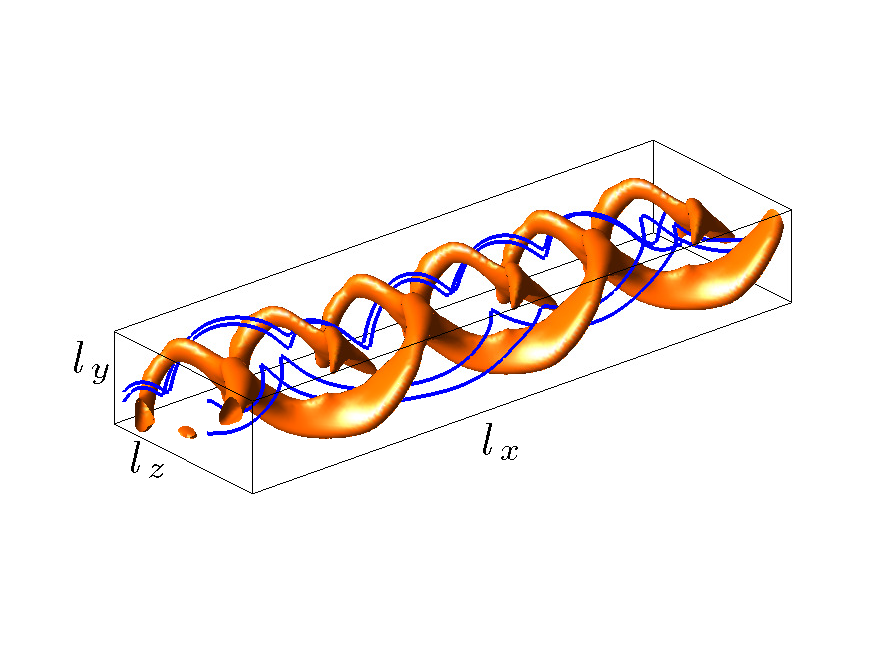
\includegraphics[width=0.5\textwidth]{example2structure3d}
     %\scalebox{0.6}[0.6]{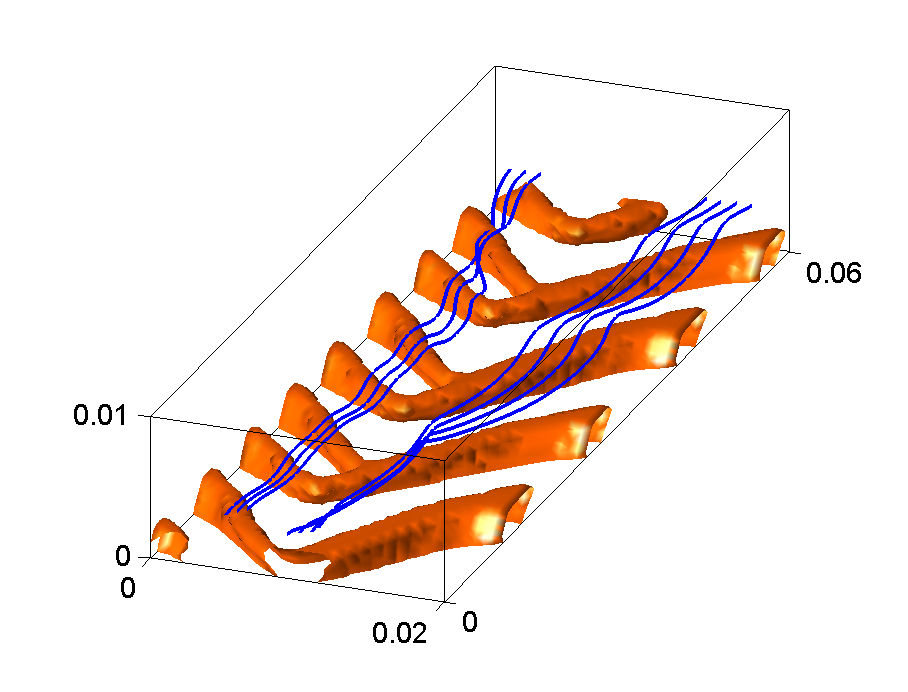
\includegraphics{myharringbonestructure}}
     %\scalebox{0.6}[0.6]{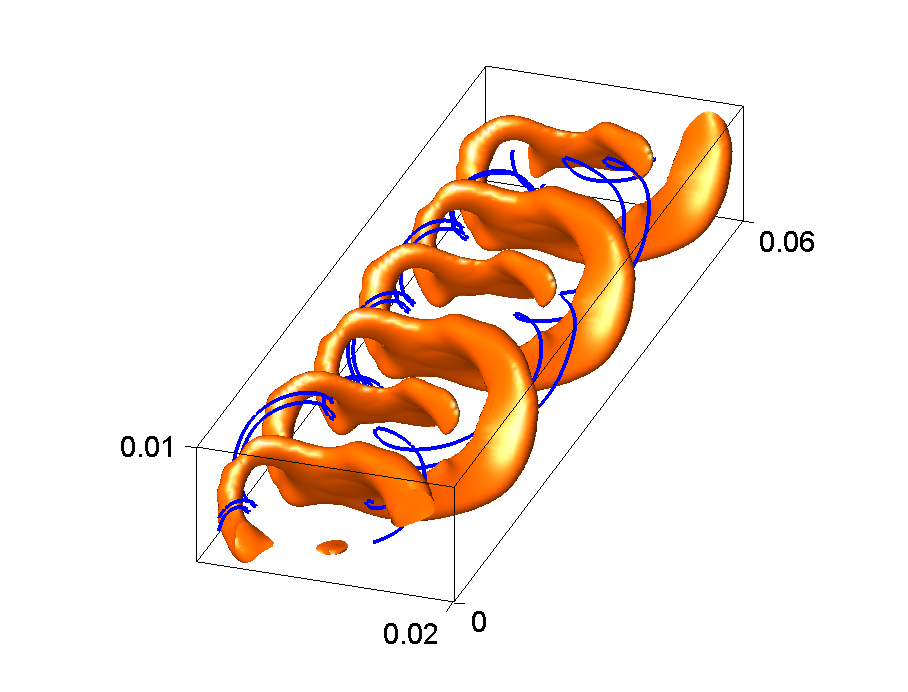
\includegraphics{my3dstructure}}
      }
    \caption{\label{example2structureNew} These two figures show the optimal channel structures to produce one big and one small vortex. For the left one we restrict the material to be on the bottom of the channel, and it forms a herringbone type structure. For the right one the material can be put anywhere inside the channel.}
  \end{figure}
%%%%%%%%%%%%%%%%%%%%%%%%%%%%%%%%%%%%%%%%%%%%%%%

%%%%%%%%%%%%%%%%%%%%%%%%%%%%%%%%%%%%%%%%%%%%%%%
%mixing trajectory
  \begin{figure}
    \centerline{
     %\scalebox{0.5}[0.5]{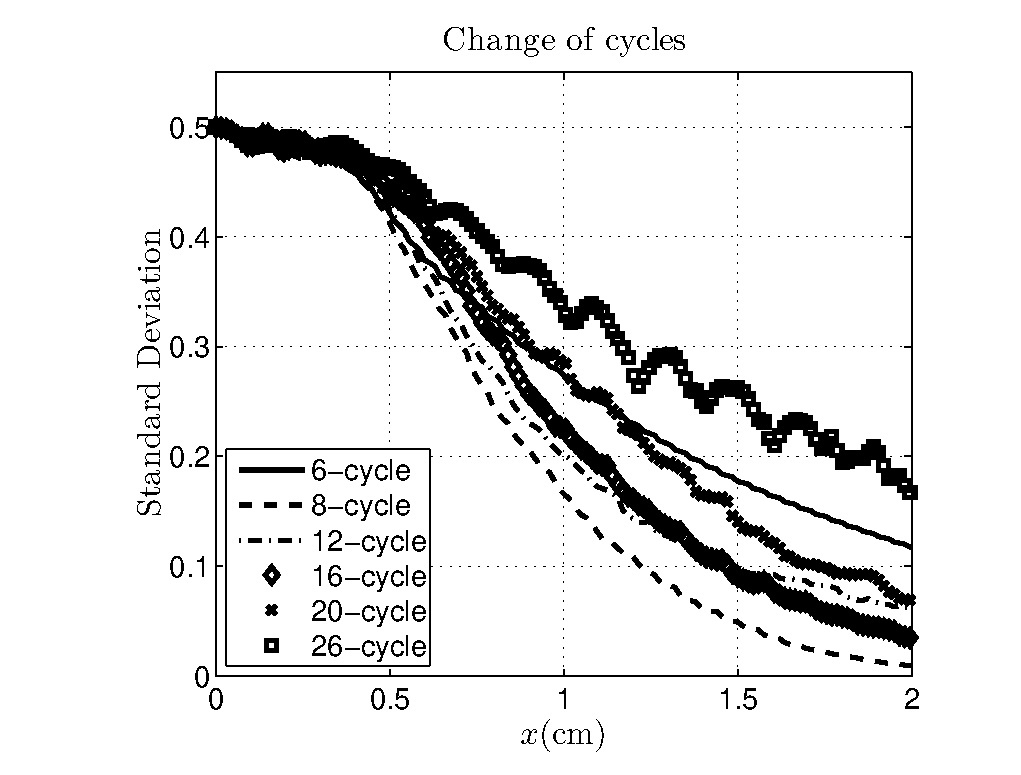
\includegraphics{example2veryCycles}}
     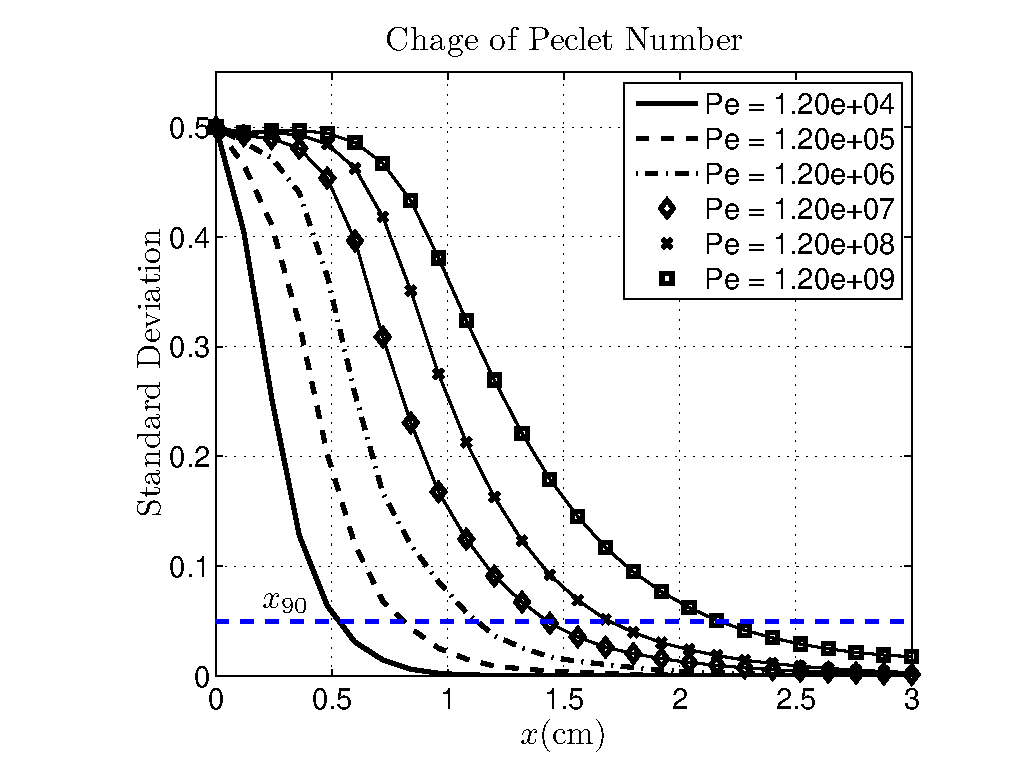
\includegraphics[width=0.58\textwidth]{example2veryPe2}}
    \caption{\label{example2trajectory} In this figure we vary $\text{Pe}$ by changing $D$ and use the $8$-cycle optimal herringbone structured channel for simulation. The mixing trajectories stay almost $0.5$ for a longer distance when $\text{Pe}$ is large.}
  \end{figure}
%%%%%%%%%%%%%%%%%%%%%%%%%%%%%%%%%%%%%%%%%%%%%%%

%%%%%%%%%%%%%%%%%%%%%%%%%%%%%%%%%%%%%%%%%%%%%%%
%cross-section simulation 1, for different Pe
  \begin{figure}
    \centerline{
     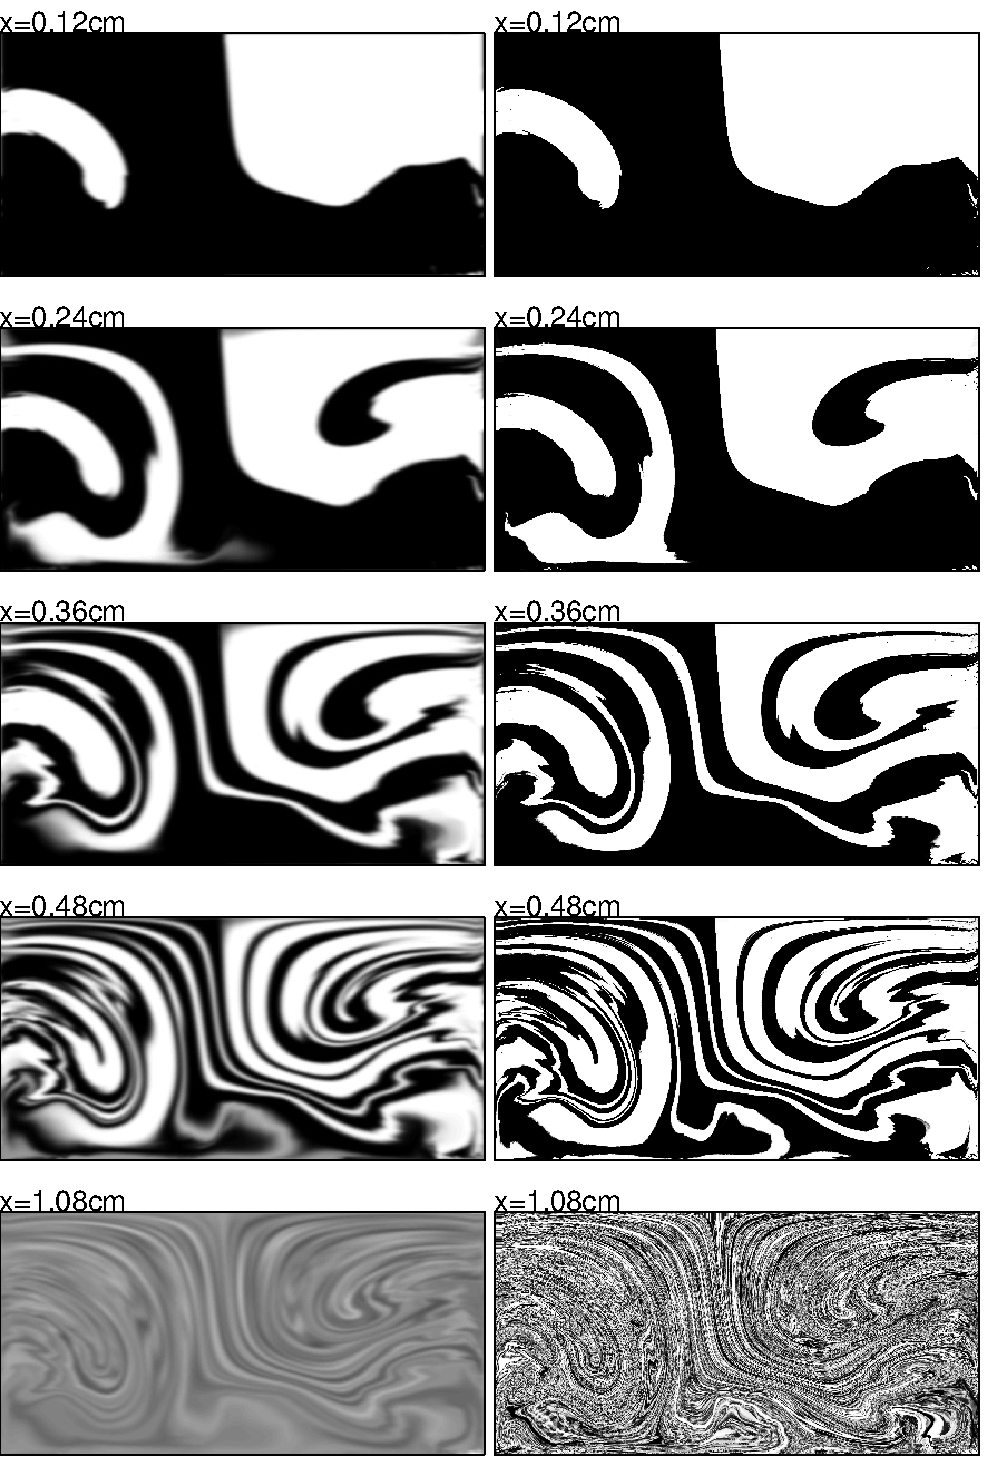
\includegraphics[width=1\textwidth]{example2simu2} 
    }
    \caption{\label{example2simu} For $\text{Pe} = 1.2\times10^6$ (left) and
$1.2\times10^9$ (right), we plot the cross-sections of the end of the
1st to the 4th cycle for both cases. The bottom two plots show the
cross-sections of the end of the 9th cycle for both cases. }
  \end{figure}
%%%%%%%%%%%%%%%%%%%%%%%%%%%%%%%%%%%%%%%%%%%%%%%

%%%%%%%%%%%%%%%%%%%%%%%%%%%%%%%%%%%%%%%%%%%%%%%%
% mixing length vs Pe, 4 cases
  \begin{figure}
    \centerline{
     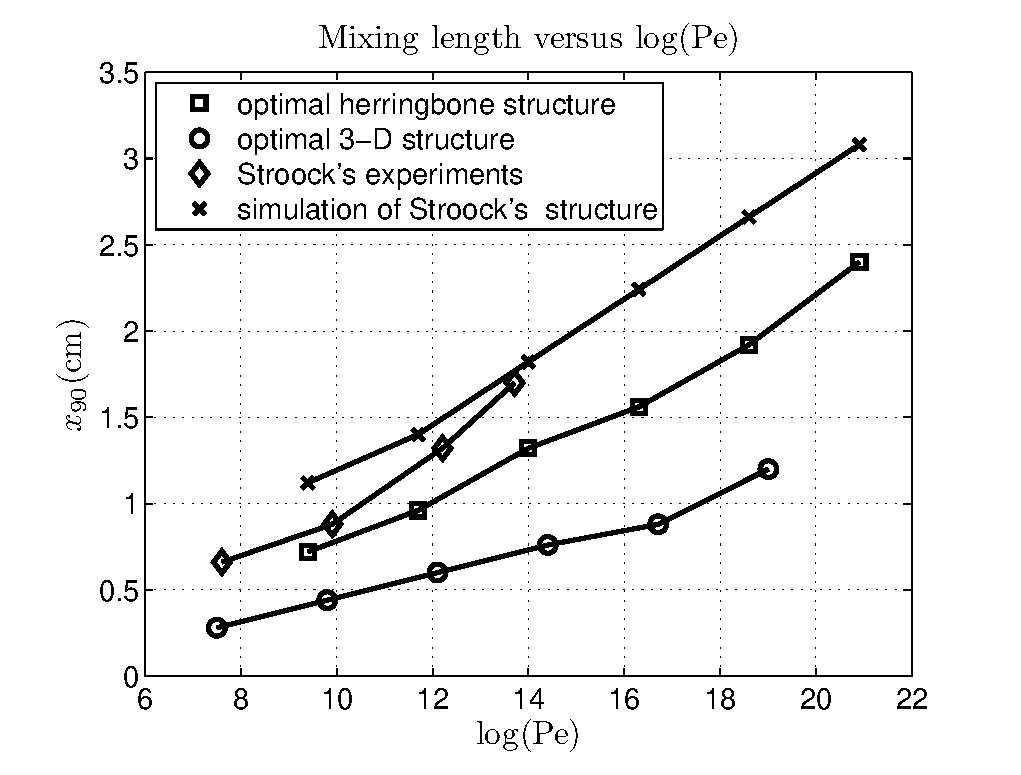
\includegraphics[width=0.58\textwidth]{example2mixinglength2}
    }
    \caption{\label{example2mixinglength} The mixing length ($x_{90}$) is defined as the
    channel length required for the standard deviation to drop from $0.5$ to $0.05$
    (see the dashed line in Figure \ref{example2trajectory}). In this figure, we plot
    $x_{90}$ versus \text{Pe} for four different cases.
  $\lozenge$: the experiment data given in \cite{Stroock2002}; $\times$: our simulation
  using the design given in \cite{Stroock2002}; $\square$: our optimal herringbone type
  mixing channel, and $\circ$: our optimal 3-D structured channel. In all cases, $x_{90}$
  grows logarithmically with $\text{Pe}$. The simulation ($\times$) agrees well with the
  experiment ($\lozenge$) when $\text{Pe}$ is large, and the two optimal designs have shorter mixing lengths compared with Stroock's design.}
  \end{figure}
%%%%%%%%%%%%%%%%%%%%%%%%%%%%%%%%%%%%%%%%%%%%%%%%

%%%%%%%%%%%%%%%%%%%%%%%%%%%%%%%%%%%%%%%%%%%%%%%%
% cross-section comparison for 3 cases.
  \begin{figure}
    \centerline{
     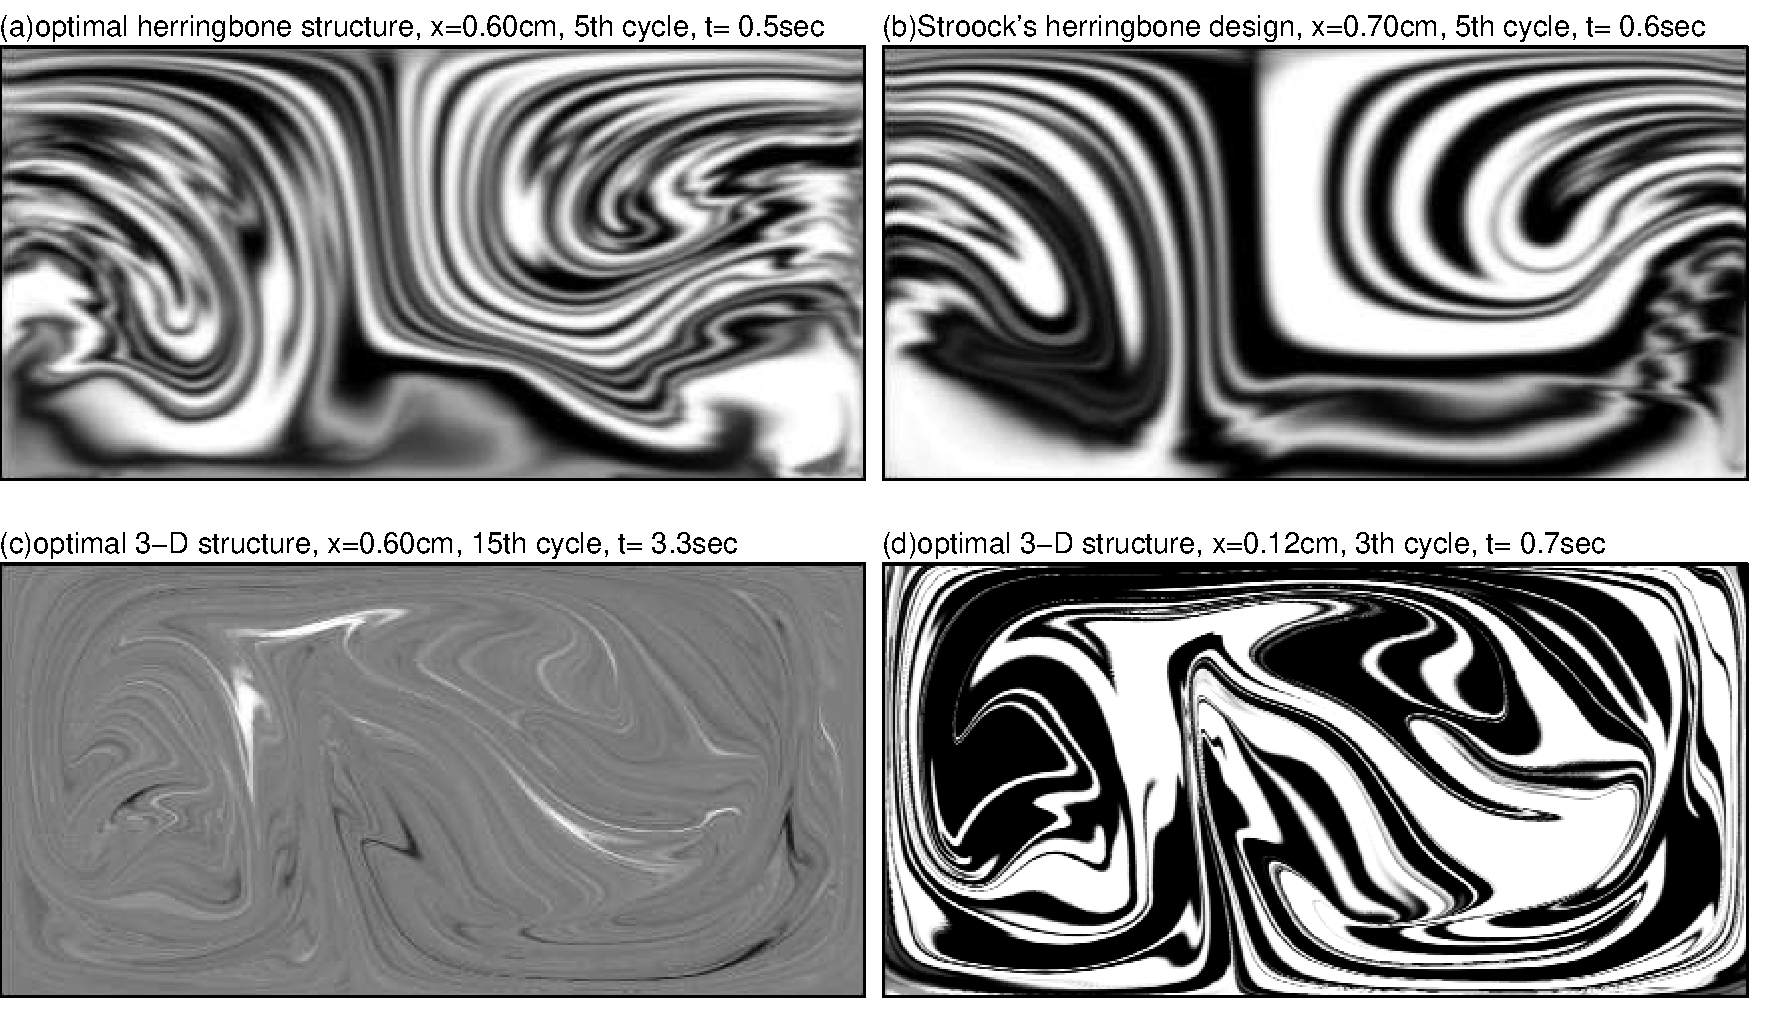
\includegraphics[width=1\textwidth]{example2crosscompare}
    }
    \caption{\label{example2crosscompare} Four cross-section plots: (a) the optimal herringbone structure at the end of its $5$th cycle; (b) the simulation of Stroock's herringbone design at the end of its $5$th cycle; (c) the optimal $3$-D structure at the end of its $15$th cycle; and (d) the optimal $3$-D structure at the end of its $3$th cycle. The color distribution in (b) is almost the same as the experimental result shown in Figure 3(C) in \cite{Stroock2002}. This demonstrates that our numerical methods are valid for simulating the true physical mixing process. Plots (c) and (d) show that although the $3$-D structure has a much smaller mixing length ($x_{90}$), it also drags the flow much more. For the same body force, the average velocity in the $x$-direction is only $1/6$ compared with the herringbone type structures. Hence for the same mixing time, the $3$-D structure is not better than the herringbone structures.}
  \end{figure}
%%%%%%%%%%%%%%%%%%%%%%%%%%%%%%%%%%%%%%%%%%%%%%%%

 % \begin{figure}
 %   \centerline{
 %    \scalebox{0.6}[0.6]{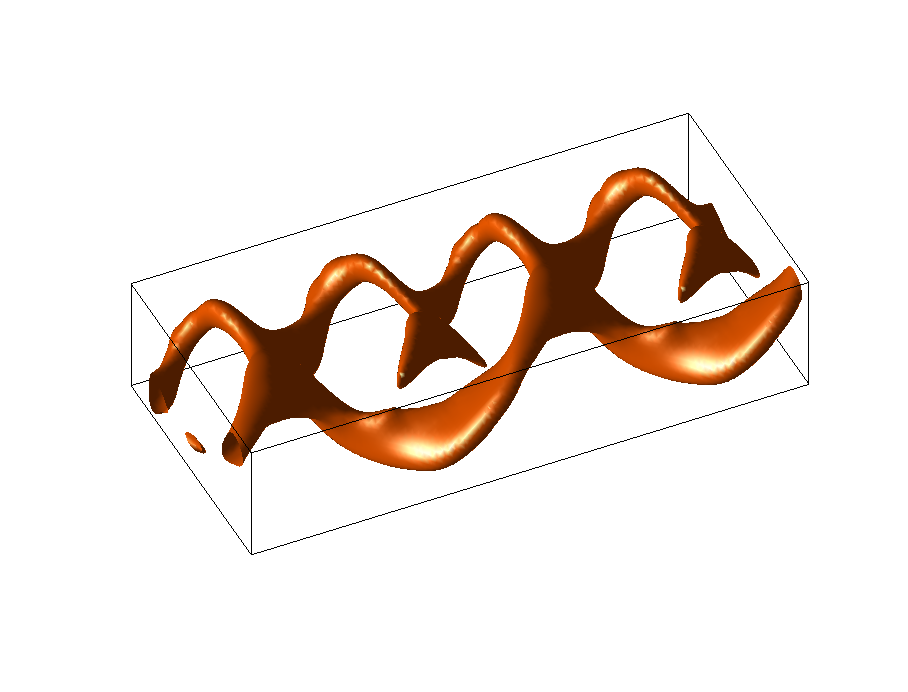
\includegraphics{example2structure}}
 %    \scalebox{0.6}[0.6]{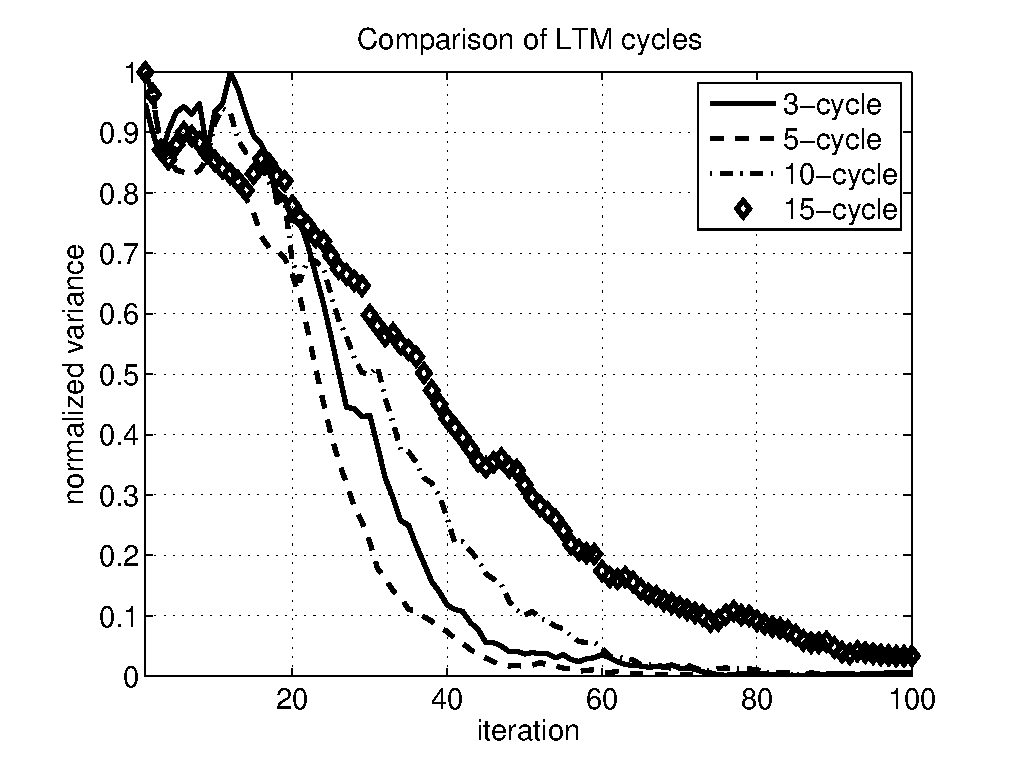
\includegraphics{ltmcompare}}}
 %   \caption{}
 % \end{figure}

 % \begin{figure}
 %   \centerline{
 %    \scalebox{0.6}[0.6]{\includegraphics{ltmsimulation}}
 %   }
 %   \caption{}
 % \end{figure}


%%%%%%%%%%%%%%%%%%%%%%%%%%%%%%%
\subsection{Designing a map}
%%%%%%%%%%%%%%%%%%%%%%%%%%%%%%%
As we have demonstrated in the previous example, the objective
function $g_1$ is really handy in the mixer design. However,
``maximizing the transverse velocity somewhere in the channel'' may
not always be a good strategy to achieve the flow we want. An ongoing
research area in chaotic mixing channel design is to realize a Linked Twist
Map. Similar to the staggered herringbone mixer, this mixing channel
is composed of two sequential regions of different channels. Each of
them is to twist the flow in a certain way and by adjusting the
arrangement of the two twist maps, one can achieve chaotic mixing. In
this type of design, we want the channel to rotate the flow for a
certain degree centered at a certain axis. The twist angle and the center
location are both important to create chaotic mixing. To realize such
a twist map, we can use the objective function $g_2$.

There are various kinds of twist maps, for example, $S(y,z;y_c,z_c,\theta): (y,z)\mapsto (y_e,z_e)$, and
\begin{align*}
   y_e &= y_c + r \cos(\alpha+\theta), \\
   z_e &= z_c + r \sin(\alpha+\theta), 
 \intertext{where}
   \alpha &= \text{atan2}(y-y_c,z-z_c), \\
   r      &= \sqrt{(y-y_c)^2 +(z-z_c)^2}.
\end{align*}
This defines a twist map centered at $(y_c,z_c)$ and with fixed
angle of rotation along the radius. This is of course not a realistic
map for a channel because it does not consider the non-slip boundary
conditions on the channel walls. However, we would like to see how far
a flow map can go. Again, the mixing channel has dimension
$(\ell_x,\ell_y,\ell_z) = (0.02,0.01,0.01)\,$cm per period, and is discretized
into $(n_x,n_y,n_z)=(64,32,32)$ grids. We use the objective function
$g_2$ for the above desired map and set $(y_c,z_c) =(0.5\ell_y, 0.5\ell_z)$.
The structure after $40$ iterations is shown in the left of Figure
\ref{example3figure1}. A set of streamlines starting from $41 \times
41$ regular mesh are calculated, and the end points, which form the
twisted grids, are plotted in the right of Figure
\ref{example3figure1}. The extra-thick line shows a block whose edges
are originally parallel to the channel walls and now rotated almost $45$
degrees. In Figure \ref{example3figure2} we show the simulation of
this channel. In the first $7$ iterations one can see how it rotates
the boundary between the colored liquids by roughly $45$ degrees. The
last plot in Figure \ref{example3figure2} shows the color field at the
$100$th iteration. Obviously, this channel does a bad job in mixing.

Unlike the objective function $g_1$, the optimal structure of this
problem is not solid. To actually fabricate this structure, porous
material is needed.

  \begin{figure}
    \centerline{
     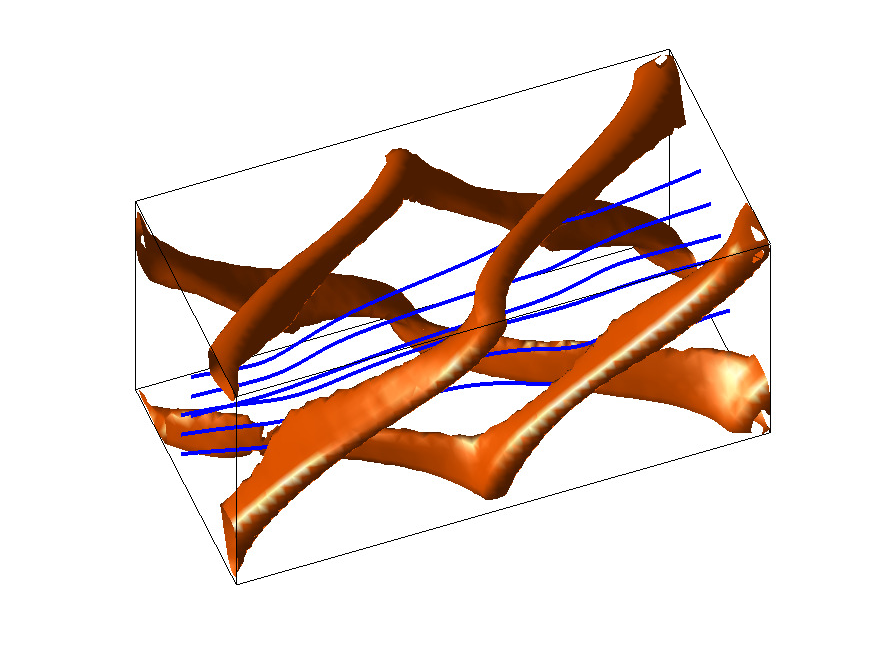
\includegraphics[width=0.5\textwidth]{example3structure}
     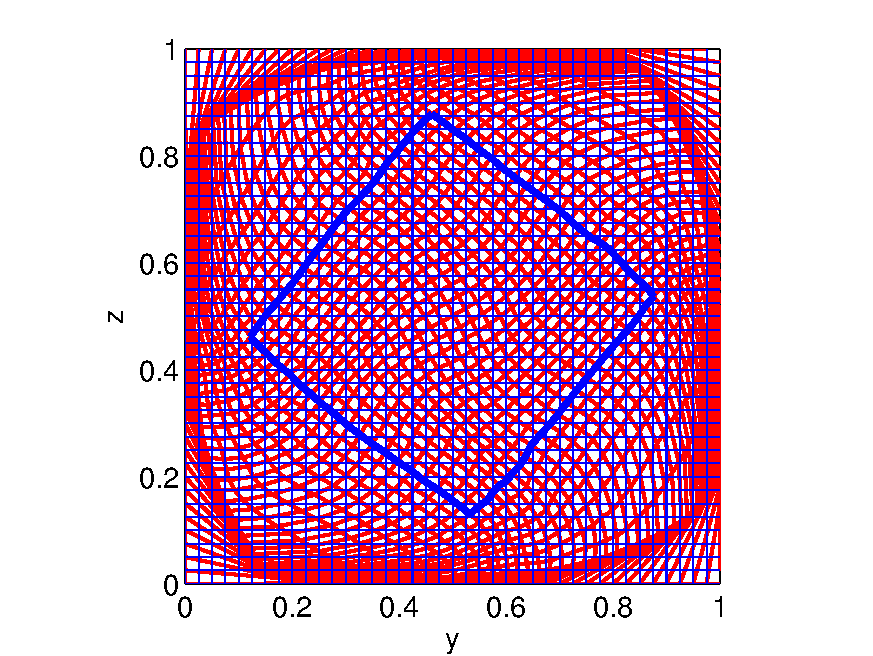
\includegraphics[width=0.5\textwidth]{example3grid}}
    \caption{\label{example3figure1} The left figure shows the optimal structure to twist the flow $45$ degrees. Note that the structure is not solid. The right figure shows the simulation of this twist channel for one period. A set of streamlines starting from $41$ by $41$ points on regular mesh grids are calculated, and the twisted grids on the other side of the channel are plotted. An extra-thick line shows a block whose edges are originally parallel to the channel boundary and now rotated roughly $45$ degrees.}
  \end{figure}


  \begin{figure}
    \centerline{
   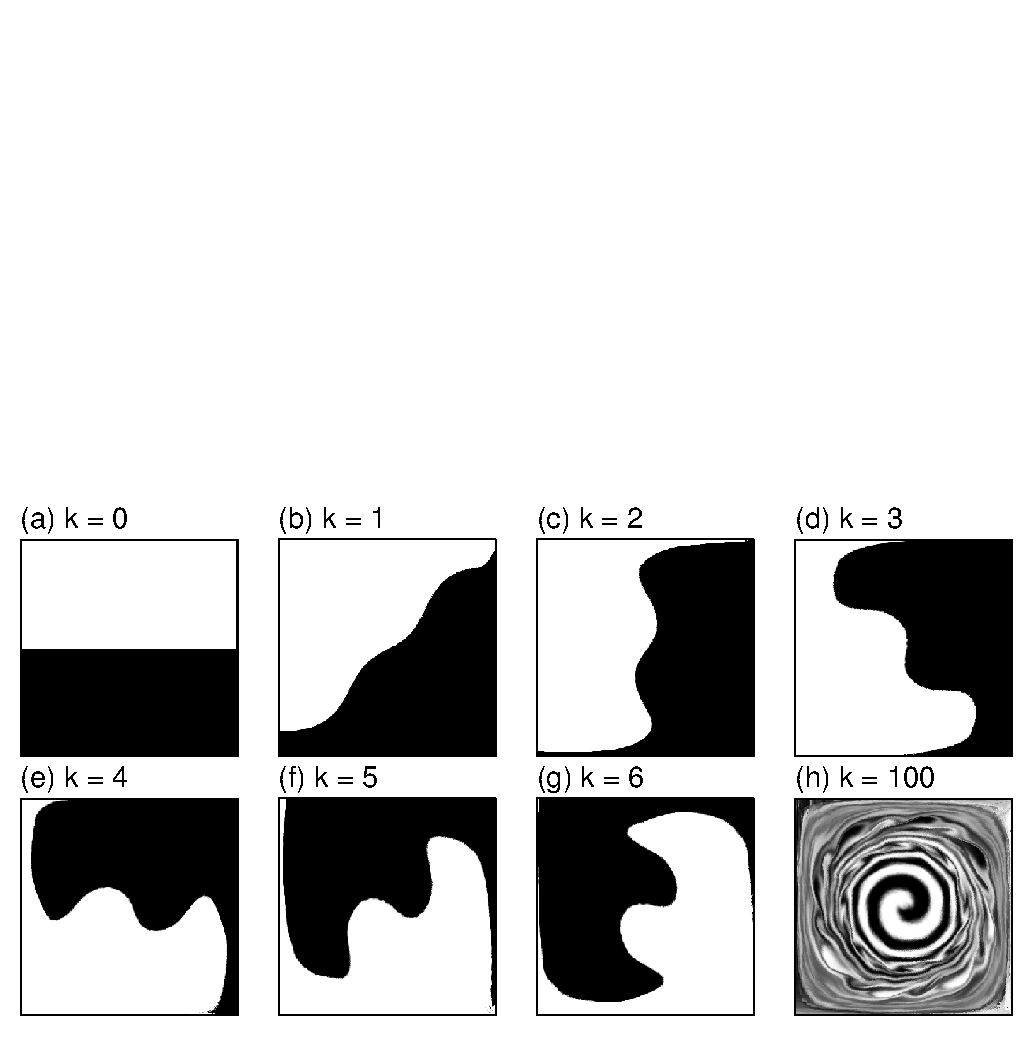
\includegraphics[width=0.9\textwidth,trim=0cm 0cm 0cm 7cm,clip]{example3simu}}
    \caption{\label{example3figure2} The simulation of the optimal structure to rotate the flow field $45$ degrees. Clearly for the first $6$ periods, the flow field is rotated $45$ degrees per period. The last plot shows the cross-section at the $100$th iteration.}
  \end{figure}

%%%%%%%%%%%%%%%%%%%%%%%%%%%%%%%%%%%%%
%\subsection{Another linked twist map}
%%%%%%%%%%%%%%%%%%%%%%%%%%%%%%%%%%%%%
%In this example we use $g_2$ objective function to design $2$ maps: $S_1(y,z;y_{c_1},z_{c_1},\theta_1)$ and $S(y,z;y_{c_2},z_{c_2},\theta_2)$, where $\{y_{c_1},z_{c_2},\theta_1\}= \{0.3\ell_y,0.3_lz,\pi/4\}$ and $\{y_{c_1},z_{c_2},\theta_1\}= \{0.7\ell_y,0.7_lz,\pi/4\}$. We find the optimal structures, and then connect them to realize a linked twist map. The connected channel is shown in figure X. The velocity field is solved again for the new channel and now the period is doubled. The simulation of this mixing channel is shown in figure X. For comparison, we also simulate the system by using each of their twist maps.
